\documentclass[11pt, a4paper, twoside]{article}

\usepackage{a4wide}
\usepackage[USenglish, ngerman]{babel}
\usepackage[latin1]{inputenc}
\usepackage[T1]{fontenc}
\usepackage{makeidx}
\usepackage{url}
\usepackage{doc}
\usepackage{graphicx}
\usepackage{lmodern} 
\usepackage{amsmath}
\usepackage{amssymb}
\usepackage{hyperref}
\usepackage{fancyheadings}
\usepackage{amsfonts}
\usepackage{amsthm}
\usepackage{color}
\usepackage{stmaryrd}
\usepackage{nomencl}
% Befehl umbenennen in abk
\let\abk\nomenclature
% Deutsche Überschrift
\renewcommand{\nomname}{Abkürzungsverzeichnis}
% Punkte zw. Abkürzung und Erklärung
\setlength{\nomlabelwidth}{.20\hsize}
\renewcommand{\nomlabel}[1]{#1 \dotfill}
% Zeilenabstände verkleinern
\setlength{\nomitemsep}{-\parsep}
\makenomenclature
\newcommand{\rf}{\color{red}}
\newcommand{\wf}{\color{white}}
\newcommand{\tf}{\color{black}}


%Kopf- und Fußzeile
\usepackage{fancyhdr}
\pagestyle{fancy}
\fancyhf{}

%Kopfzeile links bzw. innen
\fancyhead[L]{\scshape\leftmark}
%Linie oben
\renewcommand{\headrulewidth}{0.5pt}

%Fußzeile links bzw. innen
\fancyfoot[C]{\thepage}
%Linie unten
\renewcommand{\footrulewidth}{0.5pt}
\emergencystretch=3em

% Umgebungen für Sätze usw.
\newtheorem{satz}{Satz}
\newtheorem{defi}[satz]{Definition}
\newtheorem{bez}[satz]{Bezeichnung}
\newtheorem{bsp}[satz]{Beispiel}
\newtheorem{thm}[satz]{Theorem}
\newtheorem{kor}[satz]{Korollar}
\newtheorem{prob}[satz]{Problem}
\newtheorem{lem}[satz]{Lemma}

\numberwithin{equation}{section}
%\abk{DTAG}{\markup{D}eutsche \markup{T}elekom \markup{AG}}
\begin{document}


\begin{titlepage}
\pagenumbering{roman}
\begin{center}

\includegraphics[height=4cm]{hhulogo.jpg}\\
\vspace{1em}
\textbf{
\Large Heinrich-Heine-Universit"at D"usseldorf\\
\smallskip
\Large Institut f"ur Mathematik\\
\smallskip}

\vspace{3em}
{\Huge Bachelorarbeit}

\vspace{4em} {\Huge Neidfreiheit \\ \vspace{1em} in Cake-Cutting-Protokollen}
\end{center}

\vfill

\begin{center}
{\large
\begin{tabular}[l]{ll}
Name: & Alina Elterman\\
Matrikelnummer: & 1810231\\
Betreuer: & Prof. Dr. J"org Rothe\\
Abgabedatum: & 21.09.2010
\end{tabular}
}
\end{center}
\end{titlepage}
\newpage
\thispagestyle{empty}
\tableofcontents
\newpage
\pagenumbering{arabic}
\setcounter{page}{1}
\phantomsection
\thispagestyle{empty}
\listoffigures
\newpage
\section{Einleitung}
\subsection{Motivation und Aufbau}
Cake-Cutting: Was ist das eigentlich?\\
Viele Eltern q"ualen sich, wenn es darum geht, auf einem Geburtstag, gerecht den Kuchen unter den Kindern aufzuteilen. Man m"ochte alle Kinder gl"ucklich machen und jedem ein solches St"uck geben, dass es damit zufrieden ist und kein anderes haben m"ochte. Also wie l"asst sich das Problem l"osen?\\
Viele interdisziplin"are Wissenschaften, beispielweise in den Natur-,Geistes- und Wirtschaftswissenschaften versuchen eine L"osung auf die eben genannte Problematik zu geben.\footnote{Die genauen Schwerpunkte dieser Gebiete werden in Kapitel 2 aufgelistet.}\\
Doch nicht jeder Kuchen ist gleich. So kann die Form variieren und auch die M"oglichkeiten diesen zu teilen k"onnen sich unterscheiden.\footnote{Es wird eine Einf"uhrung in die M"oglichkeiten und Arten der Teilungen in Kapitel 3 gemacht.}\\
Einen Kuchen zwischen zwei Kindern aufzuteilen, ist der leichteste Fall. Dieses Verfahren nennt sich Cut \& Choose (-Protokoll) und wird im nachfolgenden ausf"uhrlich erkl"art. Bei drei Kindern birgt das mathematische Verfahren Selfridge-Conway (-Protokoll) eine L"osung.\footnote{Eine "Ubersicht der bekannten Protokolle wird in Kapitel 4 gegeben.} F"ur vier Kinder existiert eine Ausnahmeregel, f"ur f"unf konnte bis jetzt kein allgemeing"ultiges Protokoll aufgestellt werden.\\
Genau an dieser Stelle liegt eine der Problematiken dieser Arbeit. Wie l"asst sich dieser Zwiespalt l"osen?\\
Seit den 40er Jahren befassen sich verschiedene Wissenschaftler und Theoretiker mit dem Teilgebiet Cake-Cutting. Immer wieder ergibt sich die Frage nach dem gerechten Teilen. Als Begr"under und Problemsteller dieser Theorie gilt Hugo Dionizy Steinhaus mit\cite{7}(Knaster1944: bfrihbf und Steinhaus 1948). Ein weiteres Ph"anomen das sich beim Cake-Cutting bemerkbar macht, ist der Aspekt des Neides. Gamow et al. haben sich am Beispiel des  Weinteilungsproblems mit diesem Thema befasst und stellten dabei den Begriff der ''Neidfreiheit'' fest in \cite{8}.\\
In den letzten Jahrzenten wurde viel in diesem Gebiet geforscht und das Interesse von den Computerwissenschaften geweckt. Hier ist die Analyse der Komplexit"at solcher Aufteilungen prim"ar und insbesondere die Arbeit von Ariel Procaccia \cite{9} legte einen Meilenstein in der Entwicklung der Komlexit"atsanalyse.\footnote{Sie wird in Kapitel 6 beschrieben und anhand eines Beispieles demonstriert.}\\
Im Folgenden, befasst sich diese Arbeit ausf"uhrlich mit der Fragestellung von Steinhaus und den erzielten Fortschritten seiner Kollegen. Dabei wird versucht neue Ans"atze und Perspektiven zu er"offnen.
%Kapitel 7 besteht aus der Zusammenfassung mit dem Ausblick auf neue %Forschungen und einem Simulationsmodell um auf eine neue Art die %Neidfreiheit in Protokollen zu pr"ufen und vergleichen zu k"onnen.
\newpage
\section{Mehrere Ansichten der neidfreien Aufteilung}
Die gerechte Aufteilung spielt in unterschiedlichen akademischen Bereichen eine wichtige Rolle. Der Begriff der Neidfreiheit bzw. des Neides ist in diesem Kontext ebenso interdisziplin"ar. Es folgt eine "Ubersicht der Schwerpunkte  bez"uglich dieser Themen aus der Wirtschaft, Psychologie, Politik $\&$ Sozialwissenschaften, Mathematik und Informatik.\\
\textbf{Wirtschaft}
D.K.Foley hat 1967 den Begriff der Neidfreiheit eingef"uhrt. 
Interessanterweise wurde bei der Wirtschaft angefangen und intensiv an Existenzbeweisen geforscht. Es werden oft Resultate pr"asentiert die auf der Definition von Varian beruhen, dass die Gerechtigkeit gleich der Effizienz im Zusammenhang mit der Neidfreiheit (genannt Exaktheit in der Fachliteratur) sind.\\
\textbf{Psychologie}
Hier wird untersucht inwiefern individualpsychologische Faktoren oder Besonderheiten der verschiedenen Verfahren zur Aufteilung die Wahl dieser und das Ergebnis beeinflussen. Mit der Annahme nach Elster(1999), dass Emotionen und verinnerlichte Einstellungen als St"orfaktoren f"ur rationale Entscheidungen gelten wird nach "fair" empfundenen Verhandlungsl"osungen gesucht. Dabei untersucht man ausserdem das Verh"altnis der Beteiligten zueinander und die Auswirkungen der Ergebnisse und Einstellungen w"ahrend der Verhandlungen auf die Zukunft (z.B. Gebietsteilungen und Kriegsrisiko).\\ 
\textbf{Politik $\&$ Sozialwissenschaften}\\
\textbf{Mathematik}
Viele "altere Ver"offentlichungen besch"aftigen sich vor allem mit topologischen Eigenschaften (Ma"sr"aumen und auf $\sigma$-Algebren). Auch steht hier oft die Effizienz der Verteilungen im Vordergrund. Doch am wertvollsten sind die elementaren kombinatorischen Algorithmen %\footnote{$p_\aleph p_\beth p_\gimel p_\daleth$} 
und deren Analyse.\\
\textbf{Informatik}
Die gerechte Aufteilung wird als Teilgebiet der Computational Social Choice, sowie Multiagent Systems insbesondere bei Multiagent Ressource Allocation (MARA) gesehen. Von dem Letzteren unterscheidet sie sich aber in der Konzentration auf die unterschiedlichen Gerechtigkeitskriterien.\\
Die gerechte Aufteilung spaltet sich in zwei Unterbereiche, die Teilung von unteilbaren G"utern und Cake-Cutting (Teilung von beliebig teilbaren G"utern). So "ahnlich sie auch klingen m"ogen, sind die verwendeten Methoden dennoch kernunterschiedlich. W"ahrend es sich bei den unteilbaren G"utern eher um Optimierungsprobleme handelt, greift Cake-Cutting auf ganz andere mathematische Methoden zu, die in den nachfolgenden Kapitel aufgef"uhrt werden.
\newpage
\section{Grundlagen}
Bei der gerechten Aufteilung m"ussen wir zun"achst einmal alle M"oglichkeiten definieren welches Objekt, mit welchem Ziel und zwischen welchen Subjekten aufgeteilt werden kann.
\subsection{Die Spieler}
Sei $P_n$=$\{p_1,...,p_n\}$ die Menge von $n$ Spieler (oder Agenten), die ein Interesse an unserem Gut haben. Es wird angenommen, dass jeder von ihnen m"oglichst viel von der Ressource haben m"ochte.\footnote{Im Gegensatz dazu werden in der Literatur auch F"alle "uber Aufteilung von unerw"unschten Objekten (Chore Division) behandelt, z.B. zus"atzliche Arbeit, wo alle daran interessiert sind m"oglichst, wenig zu erhalten.} Au"serdem sind unsere Spieler nur an ihrem eigenen Wohl interessiert, d.h., die Verschlechterung oder Verbesserung der Situationen von ihren Mitspielern hat keinen direkten Einfluss auf ihr Wohlbefinden.
\subsection{Der Kuchen}
Wir besch"aftigen uns mit der Aufteilung von einem einzigen, heterogenen, beliebig teilbaren Gut.\footnote{Es existieren auch Forschungen "uber die Aufteilung von mehreren G"utern (z.B. \cite{1}), die wir hier aber au"ser Acht lassen.} Ein Objekt ist heterogen, wenn es uneinheitlich hinsichtlich eines oder mehrerer Merkmale ist oder wie in diesem Zusammenhang, wird ein Merkmal uneinheitlich auf dem gesammten Gut verteilt. Zur Veranschaulichung wird ein rechteckiger Kuchen (Stollen) verwendet. \footnote{Es gibt mehrere Studien von einer Torte (runder Kuchen) nachzulesen in M.A.Jones:''Some Recent Results on Pie Cutting'').} Die Division wird bei uns durch eine Reihe von parallen Schnitten durchgef"uhrt.\footnote{Es gibt ebenfalls Aufteilungen mit parallelen und rechtwinkligen Schnitten (z.B. Protokoll von Webb).} Der Kuchen $X$ wird dabei durch das Intervall $I=[0,1]\subseteq \mathbb{R}$ repr"asentiert. Wir nennen jedes Teilintervall $I'\subseteq I$, oder eine Vereinigung von solchen, ein \underline{St"uck}. Diese St"ucke sind immer disjunkt. Eine wichtige Eigenschaft von Cake-Cutting ist, dass wir nur komplette Aufteilungen, wo jedes St"uck einem Spieler zugeordnet wird, des Kuchens betrachten. Wir bezeichnen als $X_i$ das St"uck des Kuchens, welches der Spieler $p_i$ bekommt.
\subsection{Die Bewertung} 
Jeder Spieler $p_i \in P_N$ besitzt eine Bewertungsfunktion (Bewertung) $v_i:\{X'|X'\subseteq X\}\mapsto [0,1]$ des Kuchens $X$. Sie erf"ullt folgende Eigenschaften:
\begin{enumerate}
\item Nicht-Negativit"at: $v_i(C)\geq 0$ f"ur alle $C\subseteq [0,1].$
\item Normalisierung: $v_i(\emptyset)=0$ und $v_i([0,1])=1.$
\item Monotonit"at: Wenn $C' \subseteq C$, dann $v_i(C') \leq v_i(C).$
\item Additivit"at: $v_i(C \cup C')=v_i(C)+v_i(C')$ f"ur disjunkte $C,C'\subseteq [0,1].$
\item Teilbarkeit: F"ur alle $C\subseteq [0,1]$ und alle $\alpha \in \mathbb{R}$, $0\leq \alpha \leq 1$, existiert ein $B\subseteq C$, so dass  $v_i(B)=\alpha \cdot v_i(C).$
\item  $v_i$ ist kontinuierlich: Falls $0<x<y\leq 1$ mit $v_i([0,x])=\alpha$ und $v_i([0,y])=\beta$, dann gilt f"ur jedes $\gamma \in [\alpha,\beta]$ existiert ein $z \in [x,y]$ so dass $v_i([0,z])=\gamma.$
\item Inhaltslosigkeit von Punkten:  $v_i([x,x])=0$ f"ur alle $x\in [0,1].$
\end{enumerate}
Au"serdem wird "ublicherweise verlangt, dass jede nicht leere Teilmenge des Kuchens auch einen positiven Wert f"ur jeden Spieler besitzt.\\
Folgend werden zwei unterschiedliche Darstellungen f"ur den Kuchen und deren Bewertung genutzt.\\
\newline
Die \textbf{Boxendarstellung}:\\
 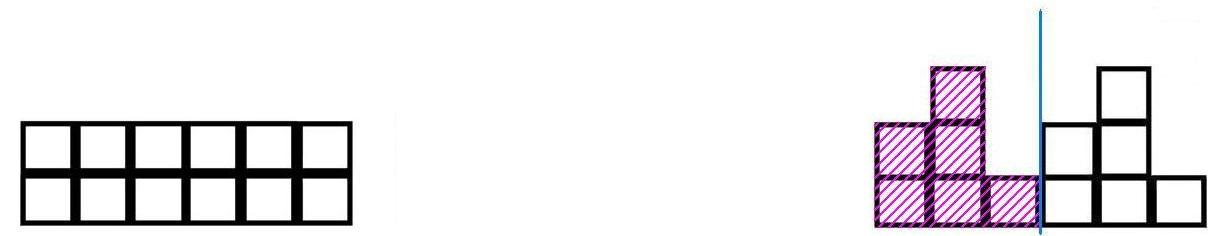
\includegraphics[height=3cm]{cc1svv.jpg}\\
Eigenschaften: Ein solches Diagramm muss separat f"ur jeden Spieler erstellt werden. Die Anzahl der K"astchen ist bei allen Spielern gleich und diese repr"asentieren immer den gleichen Wert des Kuchens. Ab hier wird der Wert des Kuchens pro K"astchen genau $1/12$. Der objektive Wert eines Kuchens sieht wie die linke Abbildung aus. Es werden die 12 K"astchen nach der jeweiligen Bewertung des Spieler verteilt, wie z.B. in der rechten Abbildung. Die straffierte Fl"ache ist das St"uck, welches der jeweilige Spieler erh"alt und dessen Summe ist der Wert seines St"uckes. Die parallelen Schnitte werden wie abgebildet eingezeichnet.
\subsection{Die unterschiedlichen Arten von Gerechtigkeit}
Wie oben bereits definiert wurde, besitzt jeder Spieler eine Bewertungsfunktion. Diese Funktion ist geheim und subjektiv (ein Spieler kennt nur seine Bewertungen, und nur seine Bewertungen haben Einfluss auf sein Wohlbefinden). Nach einer Aufteilung versuchen wir die G"ute dieser zu messen. Damit brauchen wir aber Ma"sst"abe. Das Wichtigste ist die Gerechtigkeit. Aber was bedeutet "uberhaupt gerecht? Dies ist eine philosophische oder psychologische Frage und kann nicht so einfach und f"ur unser Ziel zufriedenstellend beantwortet werden, somit brauchen wir Kriterien um unsere Aufteilungen vergleichen und bewerten zu k"onnen. Alle Kriterien sind subjektive Einsch"atzungen und keine objektiven Ma"sst"abe. 
\begin{defi}{\textbf{(Proportionalit"at oder einfache Gerechtigkeit)}}
\newline Eine Aufteilung ist \underline{proportional (einfach gerecht)}, falls  $v_i(X_i) \geq 1/n$ f"ur jeden Spieler $p_i \in P_N$ gilt. 
\end{defi} 
\begin{defi}{\textbf{(Neidfreiheit)}}
\newline Eine Aufteilung ist \underline{neidfrei}, falls $v_i(X_i) \geq v_i(X_j)$ f"ur jedes Paar von Spielern $p_i, p_j \in P_N$. 
\end{defi}
Es gibt st"arkere Einschr"ankungen f"ur diese zwei Kriterien. Ich werde diese an dem Beispiel der Neidfreiheit demonstieren.
\begin{defi}{\textbf{(Starke Neidfreiheit)}}
\newline  Eine Aufteilung ist \underline{stark-neidfrei} falls $v_i(X_i) > v_i(X_j)$ f"ur jedes Paar von Spielern $p_i, p_j \in P_N, i \neq j$.  
\end{defi} 
\begin{defi}{\textbf{(Super Neidfreiheit)}}
\newline Eine Aufteilung ist \underline{super-neidfrei}, falls $v_i(X_j) \leq 1/n$  f"ur jedes Paar von Spielern $p_i, p_j \in P_N, i \neq j$. 
\end{defi} 
\begin{defi}{\textbf{(Starke Super Neidfreiheit)}}
\newline Eine Aufteilung ist \underline{stark-super-neidfrei}, falls $v_i(X_j) < 1/n$  f"ur jedes Paar von Spielern $p_i, p_j \in P_N, i \neq j$. 
\end{defi} 
Das Problem ist, dass f"ur die st"arkeren Einschr"ankungen nicht immer Aufteilungen existieren, z.B. wenn alle Spieler die gleiche Bewertungsfunktion besitzen. 
\begin{defi}{\textbf{(Exaktheit)\footnote{In der Literatur wird an Stelle von Exaktheit oft der Begriff der Gerechtigkeit verwendet, was in gewissem Sinne den gesamten Konzept der Begriffe widerspricht, da wir alle diese Kriterien einzeln als Ma"sst"abe von gerecht befinden.}}}
\newline Eine Aufteilung ist \underline{exakt}, falls $v_i(X_i) = v_j(X_j)$ f"ur jedes Paar von Spielern $p_i, p_j \in P_N$.
\end{defi}
In wirtschaftlichen Texten werden Aufteilungen, die gleichzeitig exakt und neidfrei, sind oft als besonders gerecht empfunden. Dennoch hat die Exaktheit sogar in Kombination mit der Proportionalit"at keinen direkten Zusammenhang mit der Neidfreiheit, wie man sich am folgenden Beispiel leicht veranschaulichen kann.\\
\begin{bsp}Die Spieler Aleph, Beth und Gimel teilen einen Kuchen. Am Ende bekommt jeder Spieler genau $1/3$ des Kuchens (nach seinem Ma"s). Diese Aufteilung ist exakt und proportional. Doch Aleph ist der Meinung, dass Beths St"uck genau die H"alfte des Kuchens ist und beneidet Beth. Damit ist die Aufteilung nicht neidfrei.\end{bsp}
\textbf{Zusammenh"ange der Gerechtigkeitskriterien:}
\begin{lem}
F"ur alle Aufteilungen gilt:
\begin{enumerate}
\item Falls eine Aufteilung neidfrei ist, so ist sie auch proportional.
\item F"ur zwei Spieler ist eine Aufteilung proportional genau dann, wenn sie neidfrei ist.
\end{enumerate}
\end{lem}
\begin{proof}\wf jhbfd \tf
\begin{enumerate}
\item Beweis durch Widerspruch:\\ Sei $A$ eine Aufteilung die neidfrei, aber nicht proportional ist. Da die Aufteilung $A$ neidfrei ist, gilt $v_i(X_i) \geq v_i(X_j)$ f"ur jedes Paar von Spielern $p_i, p_j \in P_N$ und somit hat jeder Spieler mind. soviel wie jeder Andere, damit hat ein Spieler mindestens genauso viel wie $(n-1)$ Andere und damit kriegt Jeder mindestens $1/n$ und damit ist die Aufteilung $A$ proportional. $\lightning$\\Somit sind alle neidfreien Aufteilungen proportional.
\item ''$\Rightarrow$'' F"ur zwei Spieler ist eine Aufteilung proportional, wenn er mind. die H"alfte des Kuchens bekommt, damit kann der andere Spieler h"ochstens die H"alfte bekommen und wird nicht beneidet.\\ ''$\Leftarrow$'' Die R"uckrichtung folgt aus Zusammenhang 1.\\
\end{enumerate}
\end{proof}
\begin{defi}{\textbf{(Effizienz)}}
\newline Eine Aufteilung ist \underline{effizient (Pareto optimal)} falls keine andere Aufteilung existiert, die einem Spieler ein von ihm besser bewertetes St"uck einbringt, ohne die Situation eines anderen Spielers zu verschlechtern. 
\end{defi}
\begin{defi}{\textbf{(Ehrlichkeit)\footnote{In den letzten Jahren wurde diesem Aspekt ein  neuer Forschungshintergrund gegeben und Brams,Kilgour blabla. Doch man kann es als ein einzelnes Kriterium interpretieren.}}}
\newline Eine Aufteilung ist \underline{ehrlich}, falls es keine Bewertung gibt, bei der ein Spieler am Ende ein besseres St"uck bekommen h"atte durch Unaufrichtigkeit. 
\end{defi} 
Wir sind nur an Aufteilungen interessiert, wo die Ehrlichkeit die beste Strategie f"ur alle Spieler ist und somit allein durch den Algorithmus erzwungen wird. Oft wird dies erreicht, in dem der Spieler durch Unaufrichtigkeit in die Gefahr kommt die Garantie auf seinen fairen Anteil zu verlieren.\\
\subsection{Komplexit"atsklassen}
\subsection{Klassen von Protokollen}
Intuitive Beschreibung:(Algorithmus)
\newline In der Mathematik, Informatik und verwandten Gebieten, ist ein \underline{Algorithmus} eine effektive Methode zur Probleml"osung, ausgedr"uckt durch eine endliche Folge von Anweisungen.
\begin{defi}{\textbf{(Protokoll (Cake-Cutting-Protokoll))}}
\newline Ein \underline{Protokoll (Cake-Cutting-Protokoll)} ist ein adaptiver Algorithmus mit mehreren Spielern und folgenden Eigenschaften:
\begin{itemize}
\item{Es besteht aus Regeln und Strategien.\\ \underline{Regeln} sind Anweisungen, die gefordert werden ohne die Bewertungen der Spieler zu kennen.\\ \underline{Strategien} sind Empfehlungen, welchen der Spieler folgen muss um garantiert seinen gerechten Anteil zu bekommen.
} 
\item{Sofern ein Spieler das Protokoll befolgt, bekommt er nach einer endlichen Anzahl von Schritten ein St"uck des Kuchens, welches dem geforderten Gerechtigkeitskriterium entspricht. Dies geschieht unabh"angig von den Taten seiner Mitspieler.}
\item Jeder Spieler muss zu jeder Zeit in der Lage sein v"ollig unabh"angig von den anderen Spielern den Kuchen zu teilen (einen Schnitt zu machen).
\item Das Protokoll besitzt keine Informationen "uber die Bewertungen der Spieler, ausser denen die angefragt wurden in dem jeweiligen oder in den vorherigen Schritten. 
\end{itemize}
\end{defi}
\begin{defi}
Ein Cake-Cutting-Protokoll wird proportional, neidfrei, stark neidfrei etc. genannt, falls unabh"angig von den Bewertungsfunktionen der Spieler, jede Aufteilung entsprechend proportional, neidfrei etc., unter der Vorraussetzung, dass alle Spieler die vom Protokoll vorgegebenen Regeln und Strategien befolgen, ist.
\end{defi}
Eines der Ziele von Cake-Cutting ist solche Protokolle anzugeben.\footnote{Siehe auch Definition von \cite{3}, Robertson und Webb:''Approximating ...'' und Woeginger,Sgall:''An Aproximation Scheme...'' oder ''cc is not a piece of cake'' von magdon....}
\begin{defi}{\textbf{(endlich (diskret)/kontinuierlich)}}
\newline Ein \underline{endliches (diskretes)} Protokoll liefert eine L"osung nach einer endlichen Anzahl von Entscheidungen (Bewertungen, Markierungen,$\ldots$), dagegen muss ein Spieler bei einem \underline{kontinuierlichen} Protokoll unendlich viele Entscheidungen treffen.
\end{defi}
\begin{defi}{\textbf{(endlich beschr"ankt/endlich unbeschr"ankt))}}
\newline Ein \underline{endlich beschr"anktes} Protokoll hat eine obere Grenze von Schritten, welche im ung"unstigsten Fall betrachtet wird. Die gesamte Anzahl von Entscheidungen h"angt, wenn "uberhaupt, dann nur von der Anzahl der beteiligten Personen ab. Ein \underline{endlich unbeschr"anktes} Protokoll hat hingegen eine nicht im Voraus absch"atzbare Anzahl.
\end{defi}
Die am meisten gesuchten Protokolle sind endlich beschr"ankt, da sie am einfachsten in der Realit"at umsetzbar sind. Aber es gibt eine Art von kontinuierlich Protokollen, an denen ebenfalls Interesse besteht.
\begin{defi}{\textbf{(Moving-Knife-Protokoll)}}
\newline Ein Schiedsrichter, welcher unparteisch gegen"uber den Spielern ist und unbeteiligt an der Verteilung der St"ucke, \underline{schwenkt ein Messer kontinuierlich} von links nach rechts und macht parallele Schnitte sofern ein Spieler ''Halt!'' ruft. Bei manchen M-K-Protokollen wird der Schiedsrichter ausgelassen und nur ein Messer oder Schwert geschwungen.
\end{defi}
Bemerkung: In der Literatur (z.B.:Ulle Endriss:\cite{10} ''Lecture Notes on Fair Division'') werden manchmal kontinuierliche Protokolle nicht als Protokolle bezeichnet sondern zu neuen Klassen zusammengefasst, die von der Anzahl der Messer abh"angen. 
\begin{defi}{\textbf{(zusammenh"angend)}}
\newline Ein \underline{zusammenh"angendes} Protokoll liefert eine Aufteilung die aus genau einem zusammenh"angendem St"uck pro Spieler besteht. Hier d"urfen die St"ucke nicht geteilt und wieder zusammengesetzt werden.
\end{defi}
\begin{defi}{\textbf{(Grad der garantierten Neidfreiheit (DGEF))}}
\newline Als \underline{Grad der garantierten Neidfreiheit (DGEF)} eines bestimmten Protokolls wird die kleinste Summe von allen Spielern von der Anzahl von Verh"altnissen jedes Spielers zu einem Anderen bezeichnet, in der bei beliebigen Bewertungen des Kuchens kein Neid entstehen kann.\end{defi} 
Bemerkung: Der DGEF von neidfreien Protokollen ist $n\cdot(n-1)$.\section{Neidfreie Cake-Cutting-Protokolle}
\textbf{Bekannte Ergebnisse:}\\Bei der proportionalen Aufteilung gibt es verschiedene Protokolle f"ur beliebig viele Spieler. Eine "Ubersicht befindet sich in den B"uchern \cite{13} und \cite{14}. F"ur die Neidfreiheit benutzt man diese unter dem Aspekt des DGEF, wie in \cite{2} oder in der Simulation in Kapitel 7.\\
F"ur die exakte Aufteilung existiert nur ein Moving-Knife-Protokoll f"ur zwei Spieler.
Die neidfreie Aufteilung wurde f"ur bis zu vier Spieler im kontinuierlichen und bis zu drei Spieler im endlich beschr"ankten Fall gel"ost. Es gibt ein endliches Protokoll f"ur beliebig viele Spieler. Dieser unterscheidet sich stark von den bisherigen und ist nicht endlich beschr"ankt. Es gibt mehrere fast neidfreie L"osungen, siehe dazu Su\cite{11}:''SL:Rental Harmony'', Zeng:\cite{12}''Approximate EFP''.
\\Es folgen wichtige neidfreie Cake-Cutting-Protokolle (CCP). Dabei wird erl"autert wie die Neidfreiheit erreicht wird, begr"undet, woran eine Verallgemeinerung scheitert, und an einem Beispiel die Funktionalit"at gezeigt. Es werden nur Protokolle f"ur einen rechteckigen Kuchen mit parallelen Schnitten betrachtet.
\subsection{Zwei Spieler}
Es folgt das intuitivste und bekannteste endlich beschr"ankte CCP, das eine neidfreie Aufteilung liefert. Es werden ein Schnitt und eine Bewertung gemacht.\\
\newline
\begin{tabular}{|ll|}
\hline
&\textbf{Cut \& Choose-Protokoll}\wf ergrgrgevdffergdtdfvdjgujzgvjuvnkwgttvgvtrbr\tf\\
\hline
\textbf{$\cdot$ Schritt 1}&Spieler $p_1$ schneidet den Kuchen in zwei gleichwertige Teile\\&(nach seinem Ma"s).\\
\textbf{$\cdot$ Schritt 2}&Spieler $p_2$ sucht sich ein St"uck aus, das andere St"uck bekommt Spieler $p_1$.\\
\hline
\end{tabular}
\newline
\newline
\newline
Die Neidfreiheit wird elementar erreicht, da der erste Spieler zufrieden mit jedem der zwei St"ucke ist, und der andere Spieler das Privileg hat zu w"ahlen. Eine Verallgemeinerung ist ausgeschlossen, da das Verfahren nur dadurch funktioniert, dass der jeweils andere Spieler den Rest des Kuchens von dem jeweiligen Spieler bekommt.\\Bemerkung: Der erste Spieler kann nie mehr als die H"alfte des Kuchens bekommen.
\begin{bsp}\wf rfsdf
\begin{figure}[h!]
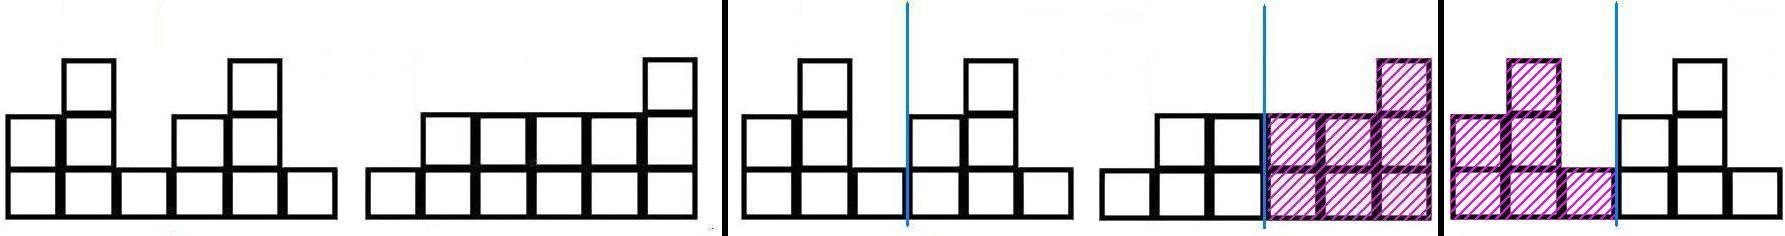
\includegraphics[height=2cm]{cc3.jpg}
\caption[Beispiel zum Cut \& Choose-Protokoll]{Boxendarstellungen des Kuchens f"ur die Spieler $p_1$ (links) und $p_2$ (rechts); Spieler $p_1$ halbiert den Kuchen(n.s.M.) (links) und Spieler $p_2$ w"ahlt das wertvollere St"uck (rechts); Spieler $p_1$ bekommt das "ubriggebliebene St"uck}
\end{figure}
\end{bsp}
Es folgt ein kontinuierlich beschr"anktes, exaktes und neidfreies CCP. Es werden h"ochstens zwei Schnitte gemacht. Dies ist das einzige bekannte exakte Protokoll.\\
\newline
\begin{tabular}{|ll|}
\hline
&\textbf{Austins Moving-Knife-Protokoll}\wf ergrgrgergegetdfvafvvvadfffrgergvtrf\tf\\
\hline
\textbf{$\cdot$ Schritt 1}& Ein Messer wird kontinuierlich von links nach rechts "uber den Kuchen\\&geschwenkt, bis ein Spieler (sagen wir: $p_1$) :''Halt!'' ruft, weil das Messer\\&den Kuchen dort halbiert (nach seinem Ma"s).\\
\textbf{$\cdot$ Schritt 2}& Dieser Spieler platziert ein zweites Messer "uber dem linken Rand des\\&Kuchens und schwenkt beide Messer parallel und kontinuierlich von links\\&nach rechts so "uber den Kuchen, dass zwischen ihnen nach seinem Ma"s\\&stets der Wert des Kuchens $1/2$ ist.\\
\textbf{$\cdot$ Schritt 3}& Der andere Spieler ruft:''Halt!'', sobald der Wert dieses St"uckes $1/2$ erreicht.\\
\hline
\end{tabular}
\newline
 Dieses Protokoll ist neidfrei, da beide Spieler genau die H"alfte des Kuchens bekommen (nach ihrem Ma"s). Die Idee hier ist: In dem Augenblick, wenn der erste Spieler ''Halt!'' ruft, ist das St"uck vom linken Rand bis zum Messer f"ur den zweiten Spieler weniger Wert als die H"alfte des Kuchens (sonst w"urde er auch:''Halt!'' rufen und damit w"are das gew"unschte Ergebnis bereits erzielt). Daraus folgt, dass das St"uck von dem Messer bis zu dem rechten Rand f"ur den zweiten Spieler mehr Wert hat als die H"alfte des Kuchens. Da der erste Spieler nun aber mit zwei Messern aus dem linken St"uck in das rechte St"uck "ubergeht, ist gesichert, dass es einen Moment gibt, wo das St"uck zwischen den beiden Messern genau die H"alfte des Kuchens f"ur den zweiten Spieler ist.\\
Um dieses Protokoll auf mehr Spieler zu verallgemeinern, muss man zeigen, dass es immer so ein St"uck geben muss, dass f"ur alle beteiligten Spieler den gleichen, oder in unserem Fall den Wert 1/2 besitzt. Das nachfolgende Beispiel 21 zeigt, dass genau dies f"ur bestimmte Bewertungen des Kuchens nicht m"oglich ist.
\begin{bsp}\wf rfsdf
\begin{figure}[h!]
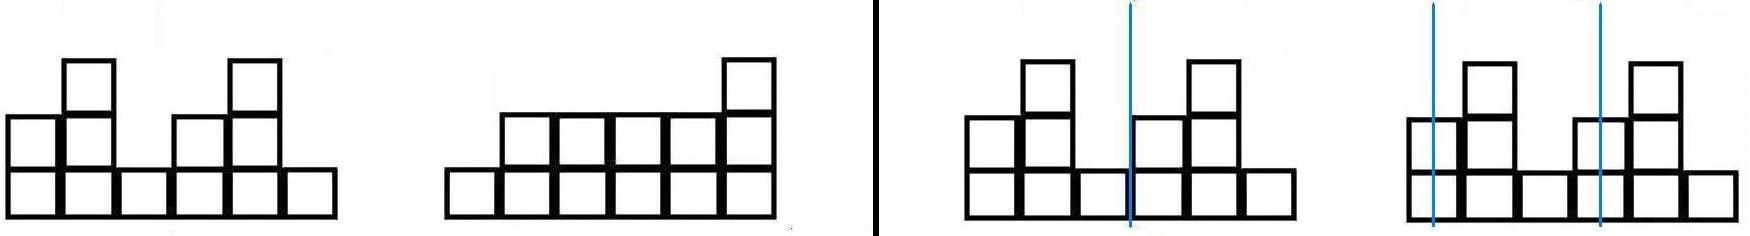
\includegraphics[height=2cm]{cc4.jpg}
\caption[Beispiel zum Austins Moving-Knife-Protokoll 1/2]{Boxendarstellungen des Kuchens f"ur die Spieler $p_1$ (links) und $p_2$ (rechts); Spieler $p_1$ ruft:''Halt!'' wenn die H"alsfte erreicht wird (links), und f"ugt ein zweites Messer hinzu und schwenkt diese "uber den Kuchen (rechts)}
\end{figure}
\begin{figure}[h!]
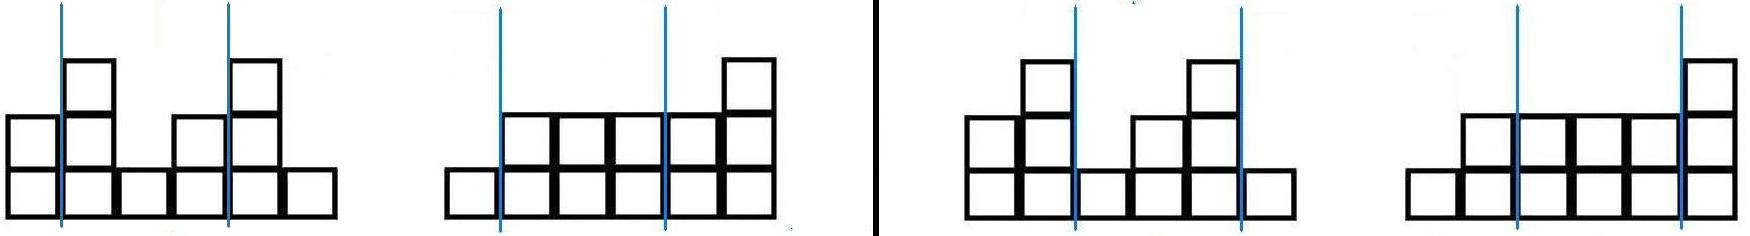
\includegraphics[height=2cm]{cc5.jpg}
\caption[Beispiel zum Austins Moving-Knife-Protokoll 2/2]{Spieler $p_2$ ruft: ''Halt!''. Beide St"ucke haben zwischen den Messern den Wert $1/2$; Die Situation in Schritt 3 ist nicht eindeutig! Der erste Zustand in dem der Wert f"ur den Kuchen f"ur beide Spieler $1/2$ ist, gilt als Ergebnis der Aufteilung.}
\end{figure}
\end{bsp}
\begin{bsp}\wf rfsdf
\begin{figure}[h!]
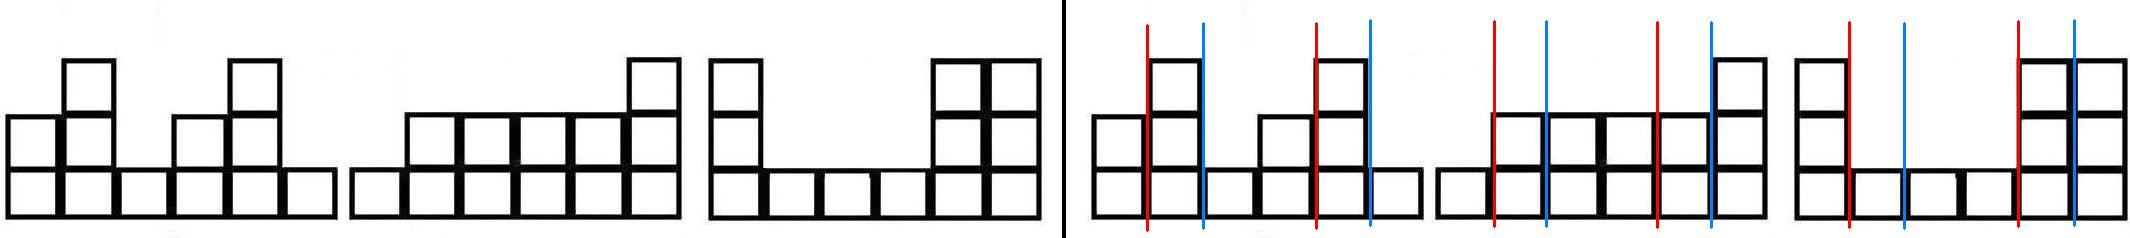
\includegraphics[height=1.73cm]{cc8.jpg}
\caption[Beispiel zum Austins Moving-Knife-Protokoll f"ur 3 Spieler]{Boxendarstellungen des Kuchens f"ur die Spieler $p_1$ (links) und $p_2$ (mitte) und $p_3$ (rechts); Man sieht das f"ur alle Aufteilungen in zwei gleiche St"ucke zwischen den Messern bei Spieler $p_1$ und $p_2$, der Spieler $p_3$ eine Bewertung kleiner 1/2 hat.}
\end{figure}
\end{bsp}  
Diese Prozedur funktioniert auch f"ur jedes beliebige $1/n$ mit $n \in \mathbb{N}$ nach der Aussage von Austin: \cite{15}, muss aber im ''worst case'' $(n-1)$- mal durchgef"uhrt werden. Da ein St"uck und die Reste aus seiner Aufteilung immer bis zum letzten St"uck "ubertragen werden m"ussen. Es folgt die Bemerkung von Austin als ausgeschriebenes Protokoll:\\
\newline
\begin{tabular}{|ll|}
\hline
&\textbf{Austins Moving-Knife-Protokoll f"ur $n$ gleichwertige St"ucke}\wf gfdffgsa\tf\\
\hline
\textbf{$\cdot$ Schritt 1}& Der Spieler $p_1$ schneidet den Kuchen in $n$ gleichwertige St"ucke (n.s.M.).\\
\textbf{$\cdot$ Schritt 2}& Der Spieler $p_2$ w"ahlt zwei St"ucke $\{X_1,X_2\}$ davon aus mit der Eigenschaft:\\&$v_2(X_1) \leq 1/n,v_2(X_2) \geq 1/n$. Alle St"ucke mit $v_2(X_i)=1/n$ f"ur $3\leq i \leq n$\\&werden als fertig markiert und stehen nicht mehr zur Wahl.\\
\textbf{$\cdot$ Schritt 3}& Diese zwei St"ucke $\{X_1,X_2\}$ werden zu einem verschmolzen und darauf\\&wird das Austins Moving Knife Protokoll angewendet. Das resultierende\\&St"uck wird ebenfalls als fertig markiert. Der Rest wird verschmolzen\\&und zu den "ubrigen unfertigen St"ucken zugeordnet, sofern einer der\\&beiden Spieler es nicht als $1/n$ bewertet.\\
\textbf{$\cdot$ Schritt 4}& Schritt 2 und Schritt 3 werden wiederholt, bis alle St"ucke markiert sind.\\
\hline
\end{tabular}
\begin{bsp}\wf rfsdf \end{bsp}
\begin{figure}[h!]
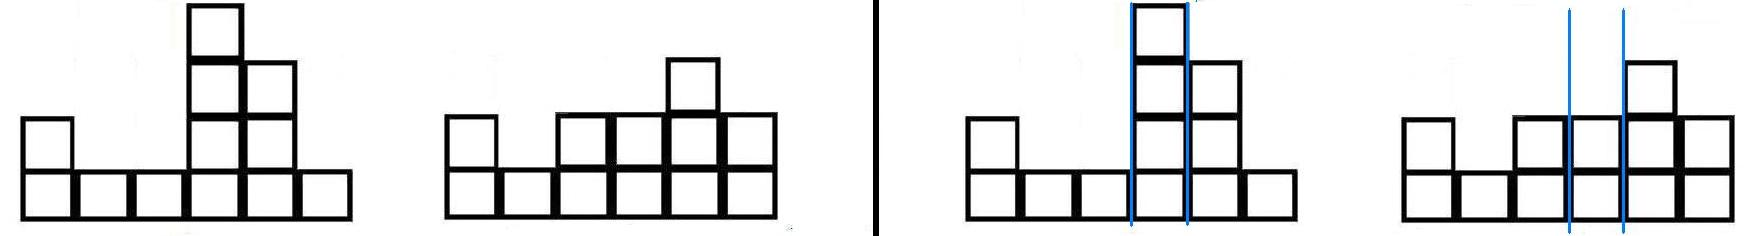
\includegraphics[height=2cm]{cc7.jpg}
\caption[Beispiel zum Austins Moving-Knife-Protokoll f"ur 3 gleichwertige St"ucke 1/2]{Boxendarstellungen des Kuchens f"ur die Spieler $p_1$ (links) und $p_2$ (rechts); Spieler $p_1$ schneidet den Kuchen in 3 gleichwertige St"ucke(n.s.M)(links)}
\end{figure}
\begin{figure}[h!]
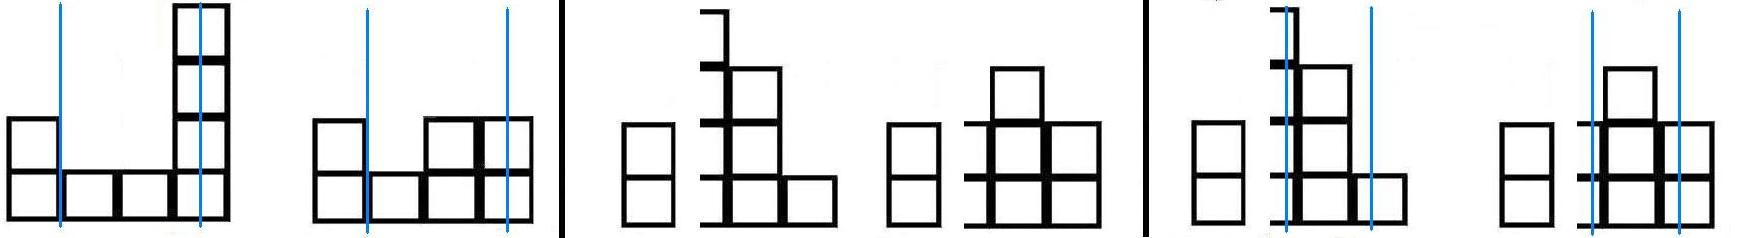
\includegraphics[height=2cm]{cc9.jpg}
\caption[Beispiel zum Austins Moving-Knife-Protokoll f"ur 3 gleichwertige St"ucke 2/2]{Spieler $p_2$ sucht sich 2 St"uckee aus mit der geforderten Eigenschaft aus Schritt 2. Beide Spieler f"uhren A-M-K-P aus; Die Reste werden "ubertragen (mitte) und A-M-K-P wiederholt ausgef"uhrt (rechts)}
\end{figure}
\subsection{Drei Spieler}
Es folgt ein endlich beschr"anktes, neidfreies CCP. Es werden h"ochstens f"unf Schnitte gebraucht. Dies ist das einzige bekannte endlich beschr"ankte neidfreie Protokoll f"ur $n \geq 3$.\\
\newline
\begin{tabular}{|ll|}
\hline
&\textbf{Selfridge-Conway-Protokoll}\wf jsngkdbfkhbdfbdfffkrgergergbdhljbfngk\tf\\
\hline
\textbf{$\cdot$ Schritt 1}&Der erste Spieler $p_1$ schneidet den Kuchen $X$ in drei gleiche St"ucke\\&(nach seinem Ma"s). Der zweite Spieler $p_2$ sortiert $\{X_1,X_2,X_3\}$ mit:\\
& $v_1(X_1)=v_1(X_2)=v_1(X_3)=1/3$ und $v_2(X_1) \geq v_2(X_2) \geq v_2(X_3)$.\\
\textbf{$\cdot$ Schritt 2}& Ist $v_2(X_1)>v_2(X_2)$, so schneidet $p_2$ von $X_1$ etwas ab, so dass er\\&$X_1'=X_1-R$ erh"alt mit   $v_2(X_1')=v_2(X_2)$. Ist $v_2(X_1)=v_2(X_2)$,\\&so sei $X_1'=X_1$.\\
\textbf{$\cdot$ Schritt 3}&Aus $\{X_1',X_2,X_3\}$ w"ahlen $p_3,p_2,p_1$ in dieser Reihenfolge je ein St"uck.\\&Wenn $p_3$ $X_1'$ nicht nimmt, muss $p_2$ es tun.\\
\textbf{$\cdot$ Schritt 4}& Entweder $p_2$ oder $p_3$ hat $X_1'$. Nenne diesen Spieler\\(nur falls $R \neq \emptyset$)&$P$, den anderen $Q$. $Q$ schneidet den Rest $R$ in drei gleiche St"ucke\\&(nach seinem Ma"s): $v_Q(R_1)=v_Q(R_2)=v_Q(R_3)=1/3 \cdot R$\\& $P,p_1,Q$ w"ahlen in dieser Reihenfolge je ein St"uck.\\
\hline
\end{tabular}
\newline
\newline
\newline
 Die erste Aufteilung von $X-R$ ist neidfrei, da der dritte Spieler die freie Wahl hat und somit keinen beneiden kann, f"ur den zweiten Spieler existieren zwei St"ucke und da er als Zweiter w"ahlen darf, ist eines davon immer vorhanden. Der erste Spieler bekommt ein unbeschnittenes St"uck und ist somit der Meinung, dass die Anderen entweder gleichgrosse oder kleinere St"ucke als er haben. Dannach wird, falls n"otig, der Rest $R$ verteilt, hier ist der erste Spieler der Meinung, dass der gesamte Rest eigentlich dem Spieler $P$ geh"ort und hat kein Problem diesen als Ersten w"ahlen zu lassen. Damit beneidet $P$ keinen, denn er durfte sich (nach seinem Ma"s) das gr"osste St"uck aussuchen. Der erste Spieler w"ahlt nun  sein St"uck und kann den Spieler $Q$ nicht benneiden. Und Spieler $Q$ ist der Meinung alle Restst"ucke waren gleich gross, und damit ist die gesamte Aufteilung neidfrei.\\
Die Verallgemeinerung scheitert vor Allem an der zweiten Aufteilung. Der erste Teil l"asst sich als das unendliche Protokoll in Kapitel 4.4 formulieren. Aber bereits hier entsteht das Problem mit den Resten. Der zweite Spieler braucht mindestens drei gleichwertige St"ucke und m"usste damit eventuell von zwei St"ucke etwas abschneiden. Damit h"atten wir mehr als einen Rest und br"auchten eine gesonderte Behandlung f"ur jeden von denen. Bei dem zweiten Teil entsteht auch das Problem, dass es zwar einen Spieler gibt, welcher der Meinung ist, dass der Rest einem bestimmten Spieler geh"ort, aber es gibt mehr als einen Spieler der dieser Meinung nicht sein muss, und somit nur neidfrei aufgeteilt werden k"onnte, wenn es m"oglich w"are f"ur mehr als \rf zwei Spieler das Austins Moving-Knife-Protokoll \tf auszuf"uhren. Eine kontinuierliche Verallgemeinerung auf vier Spieler ist das Brams,Taylors \& Zwickers Moving-Knife-Protokoll. 
\begin{bsp}\wf rfsdf
\begin{figure}[h!]
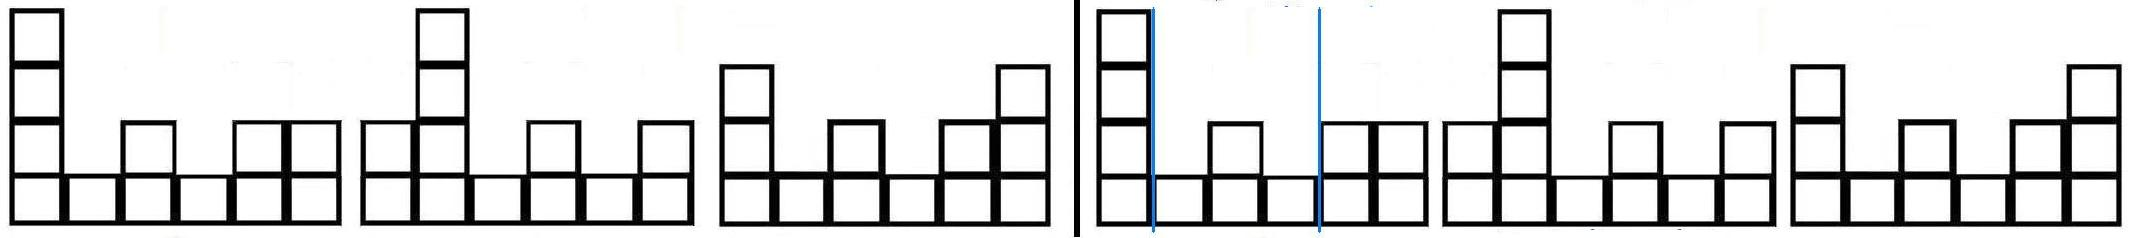
\includegraphics[height=1.73cm]{scc.jpg}
\caption[Beispiel zum Selfridge-Conway-Protokoll 1/3]{Boxendarstellungen des Kuchens f"ur die Spieler $p_1$ (links), $p_2$ (mitte) und $p_3$ (rechts); Der Spieler $p_3$ teilt den Kuchen in 3 gleichwertige St"ucke(n.s.M.)}
\end{figure}
\begin{figure}[h!]
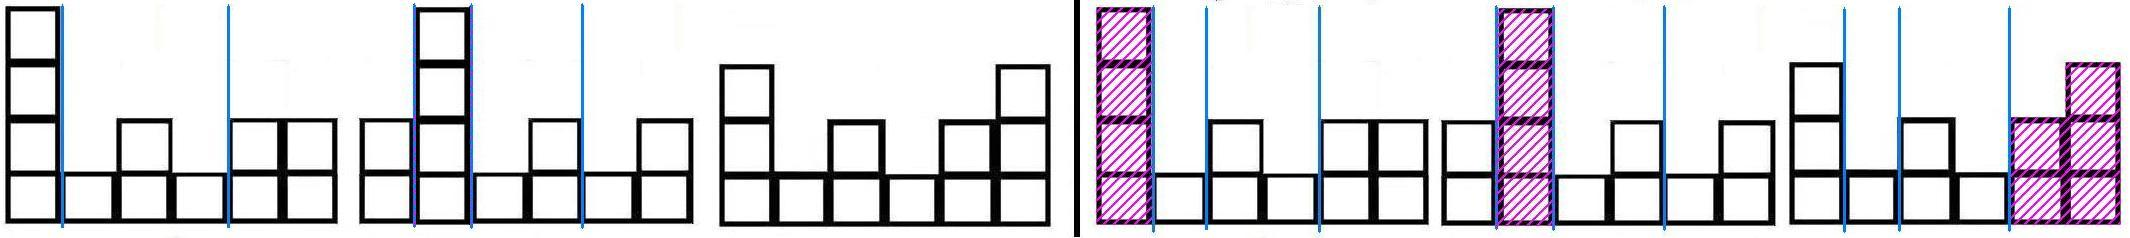
\includegraphics[height=1.75cm]{scc2.jpg}
\caption[Beispiel zum Selfridge-Conway-Protokoll 2/3]{Spieler $p_2$ schneidet den Rest von seinem wertvollsten St"uck ab; Spieler $p_3$, $p_2$ und $p_1$ w"ahlen in dieser Reihenfolge je ein St"uck}
\end{figure}
\begin{figure}[h!]
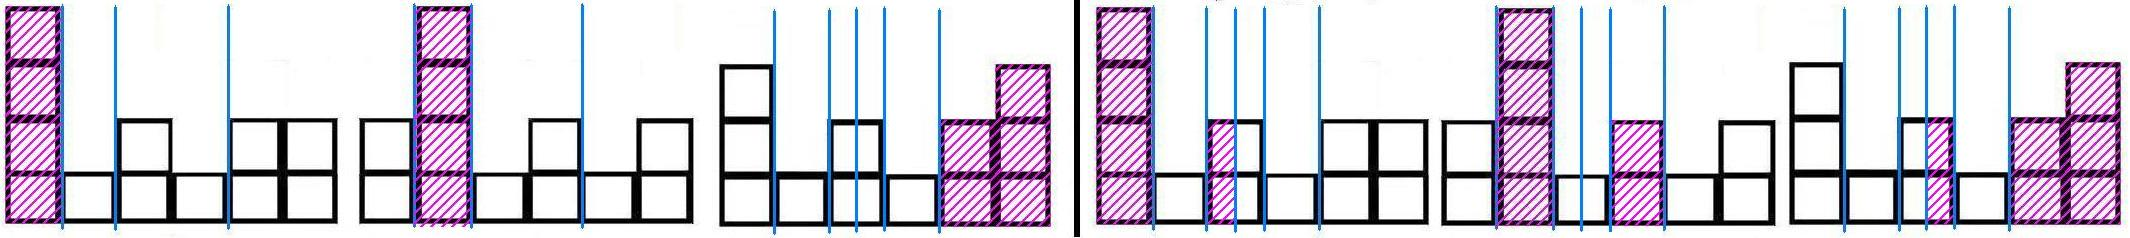
\includegraphics[height=1.75cm]{scc4.jpg}
\caption[Beispiel zum Selfridge-Conway-Protokoll 3/3]{Spieler $p_3$ unterteilt den Rest in 3 gleichwertige St"ucke (n.s.M.); Spieler $p_2$, $p_1$ und $p_3$ w"ahlen in dieser Reihenfolge je ein Restst"uck.}
\end{figure}
\end{bsp}
Es folgt ein kontinuierliches, neidfreies CCP. Es werden zwei Schnitte gemacht.\\
\newline
\begin{tabular}{|ll|}
\hline
&\textbf{Stromquists Moving-Knife-Protokoll}\\
\hline
\textbf{$\cdot$ Schritt 1}& Ein Schwert wird kontinuierlich von links nach rechts "uber den Kuchen\\&geschwenkt und teilt ihn (hypothetisch) in ein linkes St"uck $X_L$ und ein\\&rechtes St"uck $X_R$: $X=X_L\cup X_R$. Jeder der drei Spieler h"alt sein Messer\\&parallel zum Schwert und bewegt es (w"ahrend das Schwert geschwenkt\\&wird) so, dass es das rechte St"uck nach seinem Ma"s stets genau halbiert.\\&Dabei teilt das mittlere der drei Messer $X_R$ in St"ucke:$X_R=X_{RL}\cup X_{RR}$\\
\textbf{$\cdot$ Schritt 2}& Der erste Spieler, der glaubt, $X_L$ sei mindestens so gut wie sowohl $X_{RL}$ als\\&auch $ X_{RR}$, ruft: ''Halt!'' und bekommt $X_L$. Das mittlere der drei Messer\\&schneidet $X_R$ in zwei St"ucke: $X_R=X_{RL}\cup X_{RR}$. Der "ubriggebliebene\\& Spieler, der seine Markierung am n"ahesten an $X_L$ hatte, bekommt $X_{RL}$.\\&Der letzte Spieler bekommt $X_{RR}$.\\     
\hline
\end{tabular}
\newline
\newline
\newline
Um hier die Neidfreiheit nachzuvollziehen, betrachtet man jeden Spieler einzeln. Der Spieler, der ''Halt!'' ruft, ist der Meinung, dass das linke St"uck mehr oder gleich viel wert ist als jedes der beiden St"ucke rechts von dem Schwert, und wird somit auch keinen beneiden. Die "ubrigen zwei Spieler teilen seine Meinung nicht, sonst h"atten sie auch ''Halt!'' gerufen. Nun m"ussen wir die St"ucke rechts neidfrei verteilen. Es gibt drei Markierungen, als Schnitt wird die mittlere genommen. Mindestens einem der "ubrigen Spieler geh"ort eine andere Markierung, damit kriegt er ein St"uck, das sogar noch mehr wert ist und beneidet den anderen Spieler nicht. F"ur den letzten Spieler gilt entweder exakt das selbe oder er ist der Meinung genauso viel wie der Vorherige bekommen zu haben. Damit ist die gesamte Aufteilung neidfrei.\\
Die Prozedur l"asst sich leider nicht auf $n \geq 4$ "ubertragen, denn sie muss eine ungerade Anzahl von Spielern haben, um das St"uck in die entsprechenden Teile zu Markieren, oder es werden mehr als ein Schwert verlangt, was den kontinuirlichen Ablauf des Protokolls st"oren w"urde. F"ur $n=5$ tritt ein Problem in der Aufteilung der rechten St"ucke auf, da man wieder hier alle Bewertungen von Allen bis auf den Spieler, der das linke  St"uck bekommen hat beachten muss und man nicht nehr bestimmen kann, welcher Schnitt der mittlere und somit der entscheidende ist.\\ Dieses Protokoll l"asst sich nicht diskretisieren.
\begin{figure}[h!]
\center
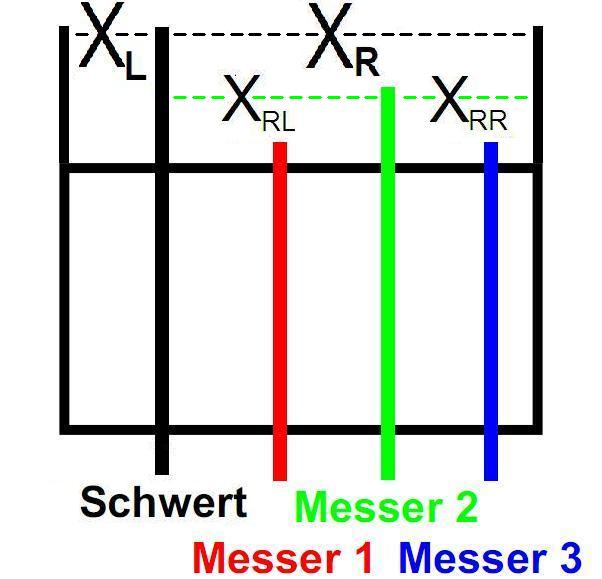
\includegraphics[height=5cm]{str.jpg}
\caption[Vorgehensweise bei Stromquists Moving-Knife-Protokoll]{Die Vorgehensweise bei Stromquists Moving-Knife-Protokoll}
\end{figure}
%\begin{bsp}\wf rfsdf
%\begin{figure}[h!]
%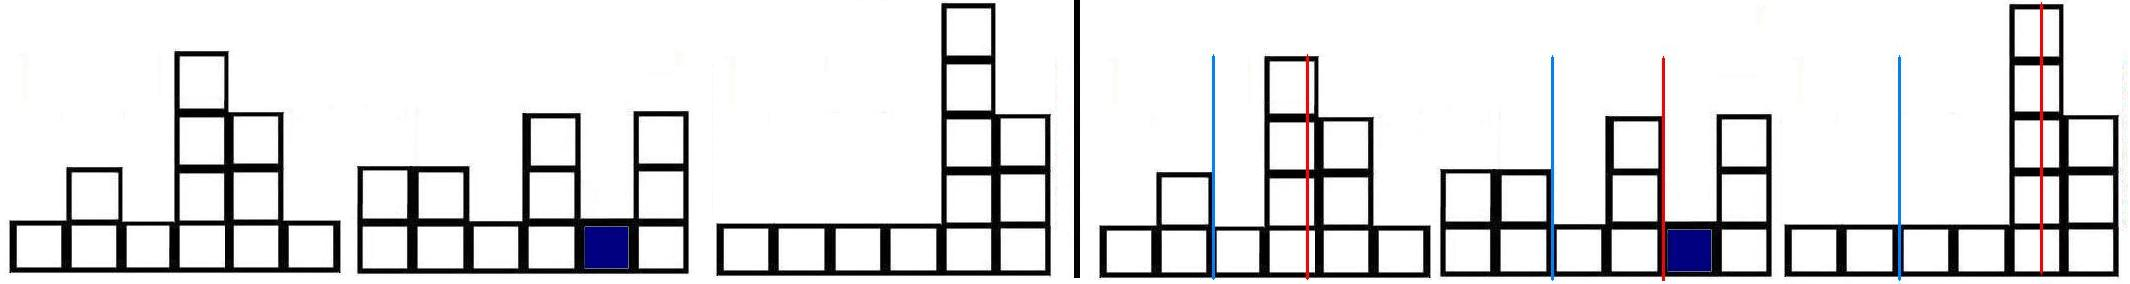
\includegraphics[height=2cm]{st2.jpg}
%\caption[Beispiel zum Stromquists Moving-Knife-Protokoll 1/2] %{Boxendarstellungen des Kuchens f"ur die Spieler $p_1$ (links), $p_2$ %(mitte) und $p_3$ (rechts); Das Schwert wird geschwenkt und die Spieler %halbieren symbolisch das rechte St"uck}
%\end{figure}
%\begin{figure}[h!]
%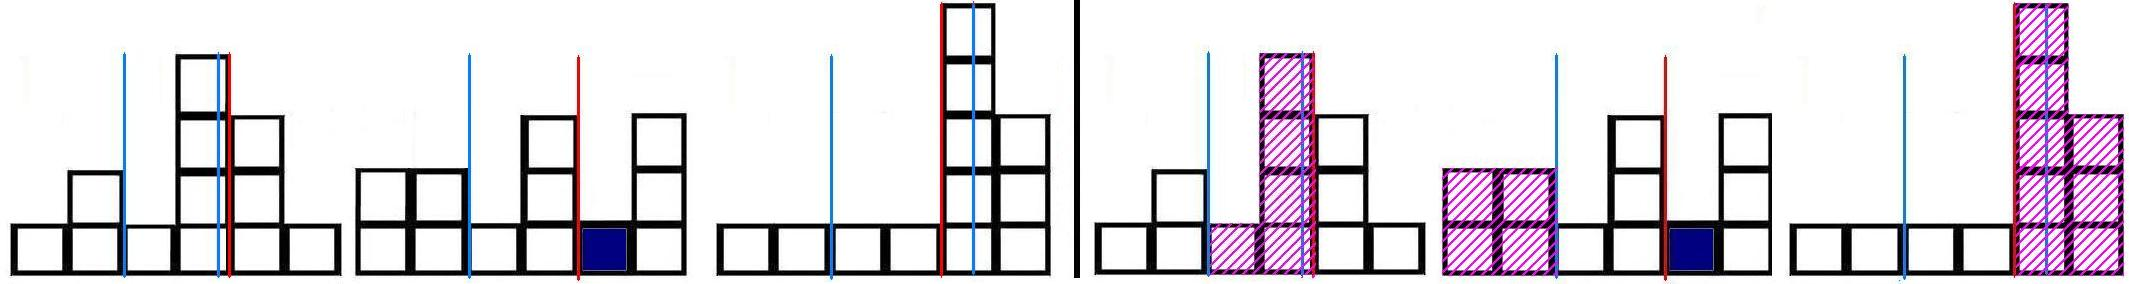
\includegraphics[height=2cm]{st4.jpg}
%\caption[Beispiel beim Stromquists Moving-Knife-Protokoll 2/2]{Spieler %$p_2$ ruft: ''Halt!''.; Die St"ucke werden nach dem Protokoll verteilt.}
%\end{figure}
%\end{bsp}
\subsection{Vier Spieler}
Es folgt ein kontinuierliches, neidfreies CCP. Es werden h"ochstens 13 (11 in\cite{16} CD with minimal cuts Barbanel $\&$ Brams) Schnitte gebraucht. Dies ist das einzige bekannte, beschr"ankte, neidfreie Protokoll f"ur $n \geq 4$.\\ 
\newline
\begin{tabular}{|ll|}
\hline
&\textbf{Brams,Taylors \& Zwickers Moving-Knife-Protokoll}\\
\hline
\textbf{$\cdot$ Schritt 1}&Der erste Spieler $p_1$ und der zweite Spieler $p_2$ erzeugen mit\\&Austins Moving-Knife-Protokoll f"ur beide Spieler vier gleichwertige\\&St"ucke. Der Spieler $p_3$ sortiert diese mit:\\
& $v_1(X_1)=v_1(X_2)=v_1(X_3)=v_1(X_4)=1/4$\\
& $v_2(X_1)=v_2(X_2)=v_2(X_3)=v_2(X_4)=1/4$\\
& $v_3(X_1)\geq  v_3(X_2)\geq v_3(X_3)\geq v_3(X_4)$\\
\textbf{$\cdot$ Schritt 2}& Ist $v_3(X_1)>v_3(X_2)$, so schneidet $p_3$ von $X_1$ etwas ab, so dass er\\&$X_1'=X_1-R$ erh"alt mit $v_3(X_1')=v_3(X_2)$. Ist $v_3(X_1)=v_3(X_2)$, so\\&sei  $X_1'=X_1$.\\
\textbf{$\cdot$ Schritt 3}&Die Spieler $p_4,p_3,p_2,p_1$ w"ahlen (in dieser Reihenfolge) je ein St"uck\\&aus $\{X_1',X_2,X_3,X_4\}$. Falls $p_4$ $X_1'$ nicht nimmt, muss $p_3$ es tun.\\
\textbf{$\cdot$ Schritt 4}& Entweder $p_4$ oder $p_3$ hat $X_1'$. Nenne diesen Spieler$P$, den anderen $Q$.\wf w\tf\\(nur falls $R \neq \emptyset$)&$Q$  und  $p_2$ schneiden den Rest $R$ mit Austins Moving-\\&Knife-Protokoll in vier gleichwertige St"ucke:\\
& $v_Q(R_1)=v_Q(R_2)=v_Q(R_3)=v_Q(R_4)=1/4 \cdot v_Q(R).$\\& $v_2(R_1)=v_2(R_2)=v_2(R_3)=v_2(R_4)=1/4 \cdot v_2(R).$\\&Die Spieler $P,p_1,Q,p_2$ w"ahlen (in dieser Reihenfolge) je ein St"uck.\\
\hline
\end{tabular}
\newline
\newline
\newline
Die Idee hier ist dieselbe wie in dem Selfridge-Conway-Protokoll. Es werden in den n"otigen Schritten immer zwei Spieler zusammengefasst um die Vorteile des Protokolls auszunutzen. Es l"asst sich aus den gleichen Gr"unden nicht verallgemeinern wie das Selfridge-Conway-Protokoll.\newpage
\begin{bsp}\wf rfsdf
\begin{figure}[h!]
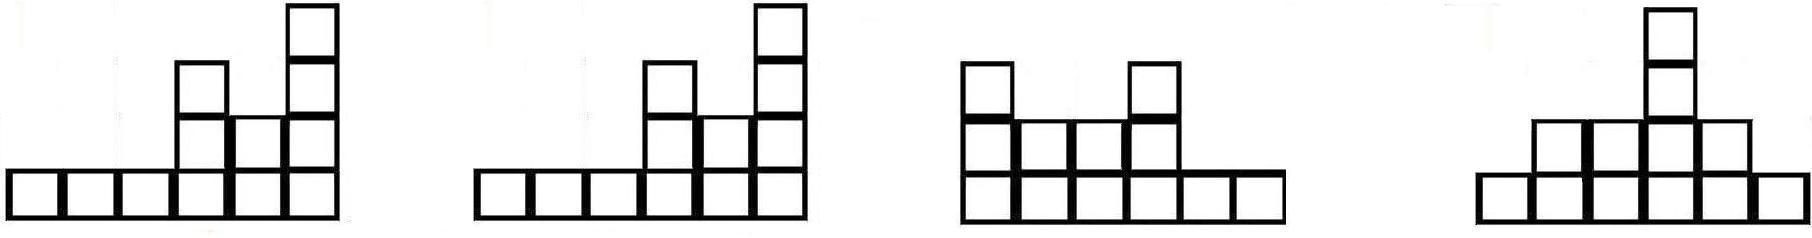
\includegraphics[height=2cm]{btz1.jpg}
\caption[Beispiel zum Brams,Taylors \& Zwickers Moving-Knife-Protokoll 1/5]{Boxendarstellungen des Kuchens f"ur die Spieler $p_1$, $p_2$, $p_3$ und $p_4$ (von links nach rechts)}
\end{figure}
\begin{figure}[h!]
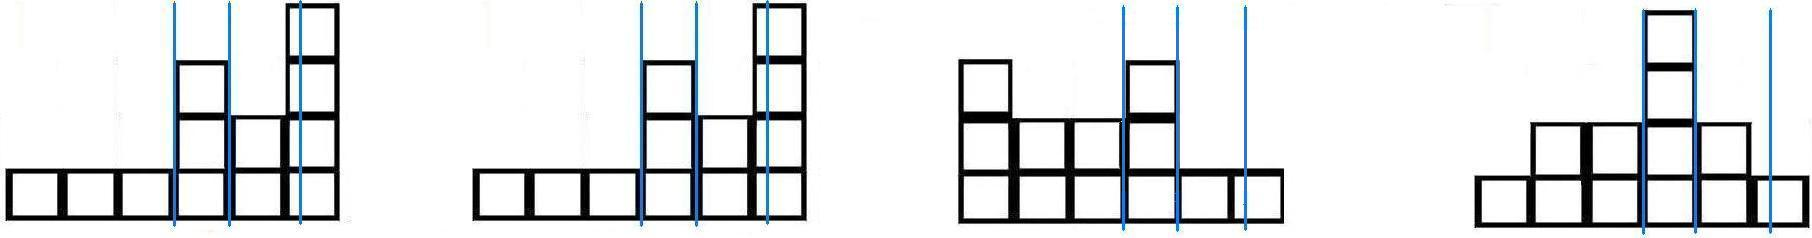
\includegraphics[height=2cm]{btz3.jpg}
\caption[Beispiel zum Brams,Taylors \& Zwickers Moving-Knife-Protokoll 2/5]{Die Spieler $p_1$ und $p_2$ teilen zusammen den Kuchen in vier gleichwertige St"ucke auf.}
\end{figure}
\begin{figure}[h!]
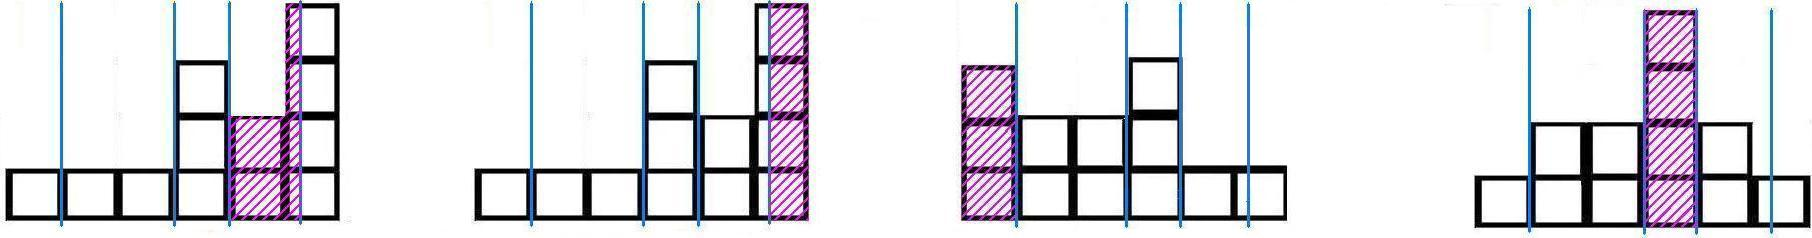
\includegraphics[height=2cm]{btz6.jpg}
\caption[Beispiel zum Brams,Taylors \& Zwickers Moving-Knife-Protokoll 3/5]{Der Spieler $p_3$ schneidet den Rest von dem wertvollsten St"uck ab (n.s.M.) und die Spieler $p_4,p_3,p_2,p_1$ w"ahlen (in dieser Reihenfolge) je ein St"uck aus.}
\end{figure}
\begin{figure}[h!]
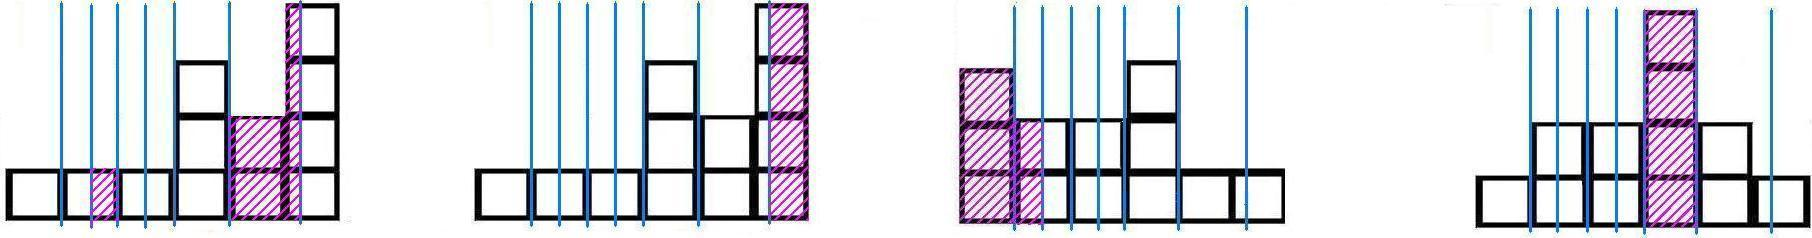
\includegraphics[height=2cm]{btz9.jpg}
\caption[Beispiel zum Brams,Taylors \& Zwickers Moving-Knife-Protokoll 4/5]{Es teilen $p_2$ und $p_4$ zusammen den Rest in vier gleichwertige St"ucke auf und die Spieler $p_3$ und $p_1$ w"ahlen (in dieser Reihenfolge) je ein Restst"uck aus.}
\end{figure}
\begin{figure}[h!]
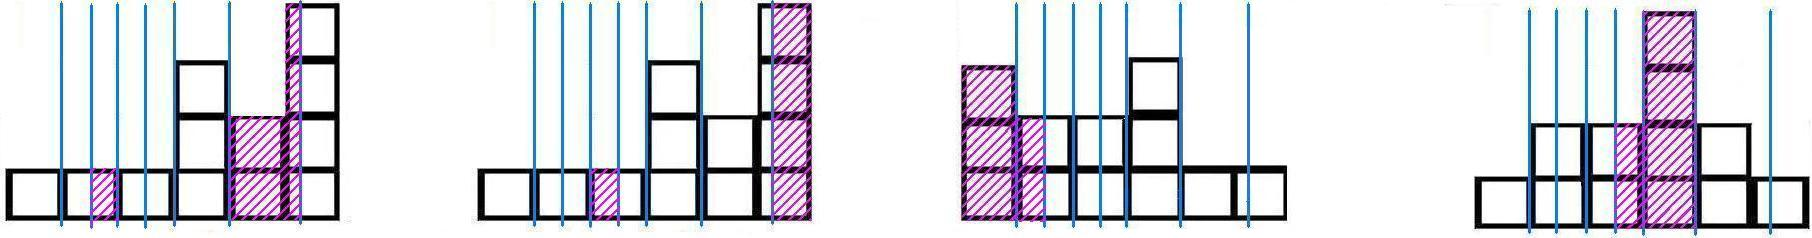
\includegraphics[height=2cm]{btz8.jpg}
\caption[Beispiel zum Brams,Taylors \& Zwickers Moving-Knife-Protokoll 5/5]{Die Spieler $p_2$ und $p_4$ nehmen je ein Restst"uck.}
\end{figure}
\end{bsp}
\subsection{$n$ Spieler}
Es existiert ein endlich unbegrenztes, neidfreies Protokoll in \cite{5} f"ur eine beliebige Anzahl von Spielern.\\
Es folgt ein unendliches neidfreies Protokoll f"ur eine beliebige Anzahl von Spielern.\\
\newline
\begin{tabular}{|ll|}
\hline
&\textbf{Ein unendliches Protokoll}\\
\hline
\textbf{$\cdot$ Schritt 1}&Der erste Spieler $p_1$ schneidet den Kuchen $X$ in f"unf gleiche St"ucke (nach\\&seinem Ma"s). Der zweite Spieler $p_2$ sortiert diese als $X_1,X_2,X_3,X_4,X_5$\wf wtw\tf\\& mit:\\
&$v_1(X_1)=v_1(X_2)=v_1(X_3)=v_1(X_4)=v_1(X_5)=1/5$\\&$v_2(X_1) \geq v_2(X_2) \geq v_2(X_3)\geq v_2(X_4)\geq v_2(X_5)$\\
\textbf{$\cdot$ Schritt 2}&Ist $v_2(X_1)>v_2(X_3)$ oder $v_2(X_2)> v_2(X_3)$, so schneidet $p_2$ ggf. von $X_1$\\&und $X_2$ etwas ab, so dass er $X_1'=X_1-R_1$ und $X_2'=X_2-R_2$ erh"alt mit   \\&$v_2(X_1')=v_2(X_2')=v_2(X_3)$. Ist $v_2(X_1)=v_2(X_3)$ oder $v_2(X_2)=v_2(X_3)$, so\\&sei $X_1'=X_1$ und $X_2'=X_2$.\\
\textbf{$\cdot$ Schritt 3}&Der dritte Spieler $p_3$ sortiert $\{X_1',X_2',X_3,X_4,X_5\}$ als $Y_1,Y_2,Y_3,Y_4,Y_5$ mit:\\
&$v_3(Y_1) \geq v_3(Y_2) \geq v_3(Y_3)\geq v_3(Y_4)\geq v_3(Y_5)$\\
\textbf{$\cdot$ Schritt 4}&Ist $v_3(Y_1)>v_3(Y_2)$, so schneidet $p_3$ von $Y_1$ etwas ab, so dass er $Y_1'=$\\&$Y_1-R_3$ erh"alt mit $v_3(X_Y')=v_3(Y_2)$. Ist $v_3(Y_1)=v_3(Y_2)$, so sei  $Y_1'=Y_1$.\\
\textbf{$\cdot$ Schritt 5}&Aus $\{Y_1',Y_2,Y_3,Y_4,Y_5\}$ w"ahlen $p_4,p_3,p_2,p_1$ in dieser Reihenfolge je ein\\&St"uck. Falls solche St"ucke noch zur Wahl stehen, muss jeder Spieler eines\\&von den St"ucken nehmen, die er selber beschnitten hat.\\
\textbf{$\cdot$ Schritt 6}&Die Reste und das "ubriggebliebene St"uck werden verschmolzen und das\\&Protokoll kann beliebig oft wiederholt werden.\\
\hline
\end{tabular}
\newline
\newline
Das folgende Protokoll l"asst sich verallgemeinern, indem die Anzahl der St"ucke in welche der erste Spieler in Schritt 1 den Kuchen teilt immer um einz gr"osser ist als die Summe der Schnitte ab Schritt 2 und bis zu dem Analogon von Schritt 5 ("ublicherweise von Schritt 2 bis Schritt 2$\cdot n$-3). Der $i$-te Spieler mit $2 \leq i \leq (n-1)$ darf immer $n-i$ St"ucke beschneiden.
\begin{bsp}\wf rfsdf
\begin{figure}[h!]
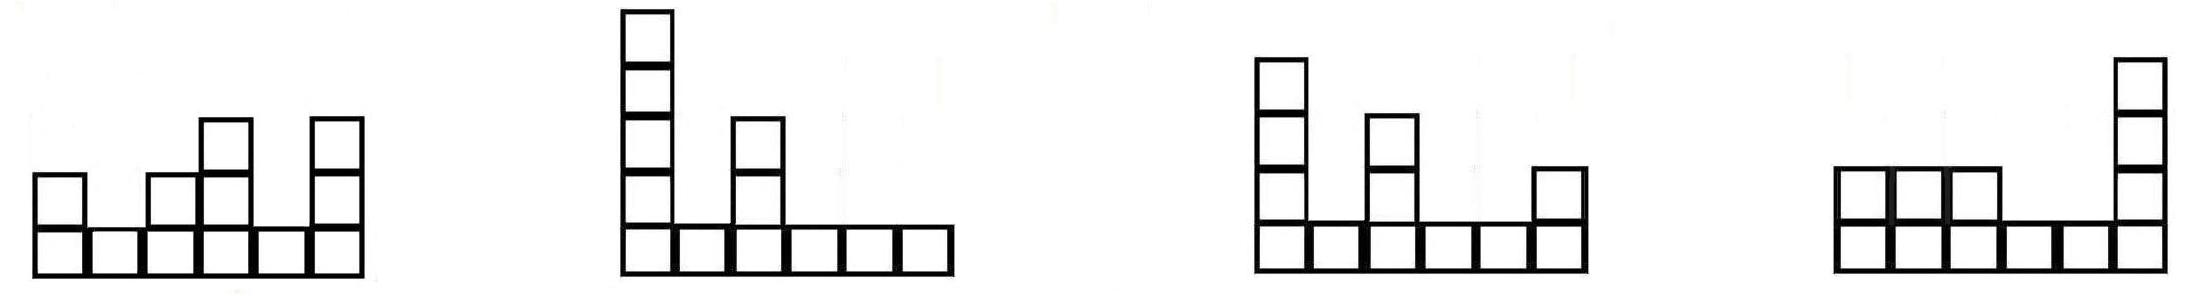
\includegraphics[height=2cm]{upfv.jpg}
\caption[Beispiel zum unendlichen Protokoll 1/4]{Boxendarstellungen des Kuchens f"ur die Spieler $p_1$, $p_2$, $p_3$ und $p_4$ (v.l.n.r.)}
\end{figure}
\begin{figure}[h!]
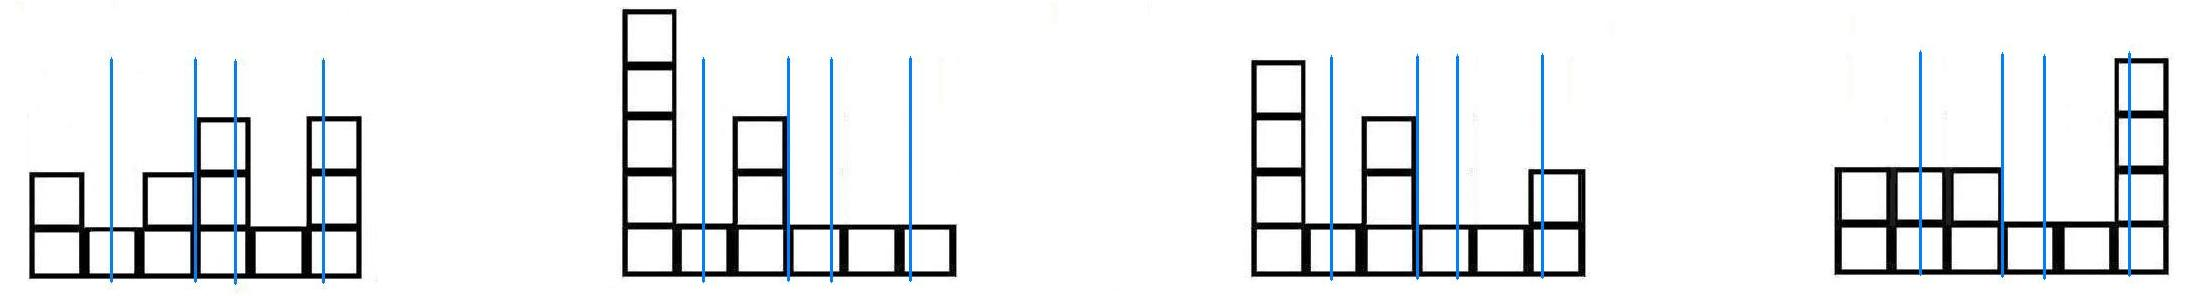
\includegraphics[height=2cm]{upfv2.jpg}
\caption[Beispiel zum unendlichen Protokoll 2/4]{Der Spieler $p_1$ viertelt den Kuchen (n.s.M.).}
\end{figure}
\begin{figure}[h!]
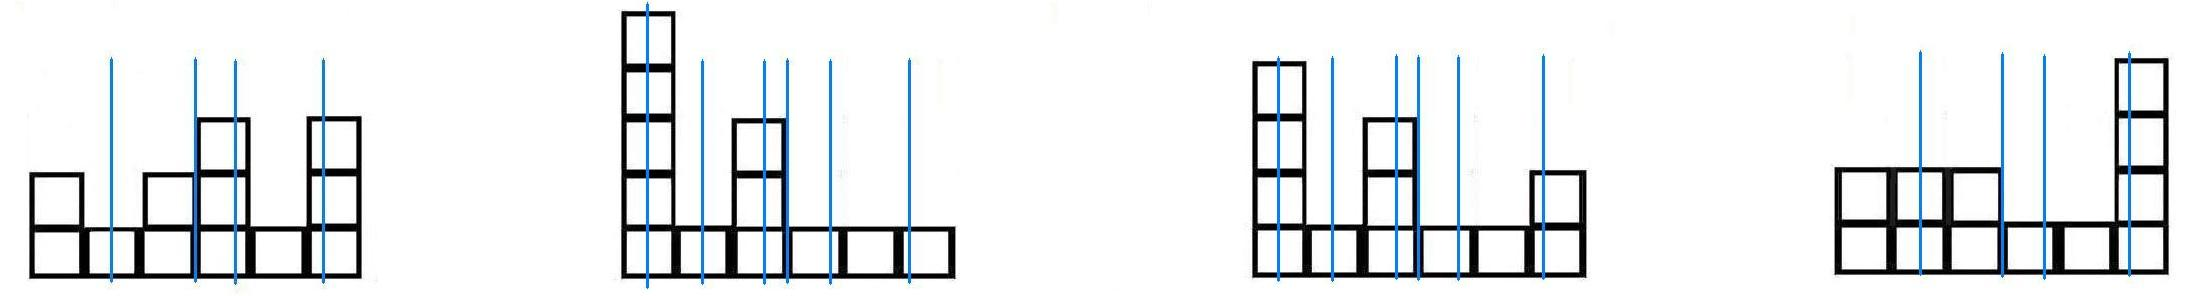
\includegraphics[height=2cm]{upfv3.jpg}
\caption[Beispiel zum unendlichen Protokoll 3/4]{Der Spieler $p_2$ schneidet je einen Rest von seinen zwei wertvollsten St"ucken. Der Spieler $p_3$ muss damit kein St"uck mehr beschneiden.}
\end{figure}
\begin{figure}[h!]
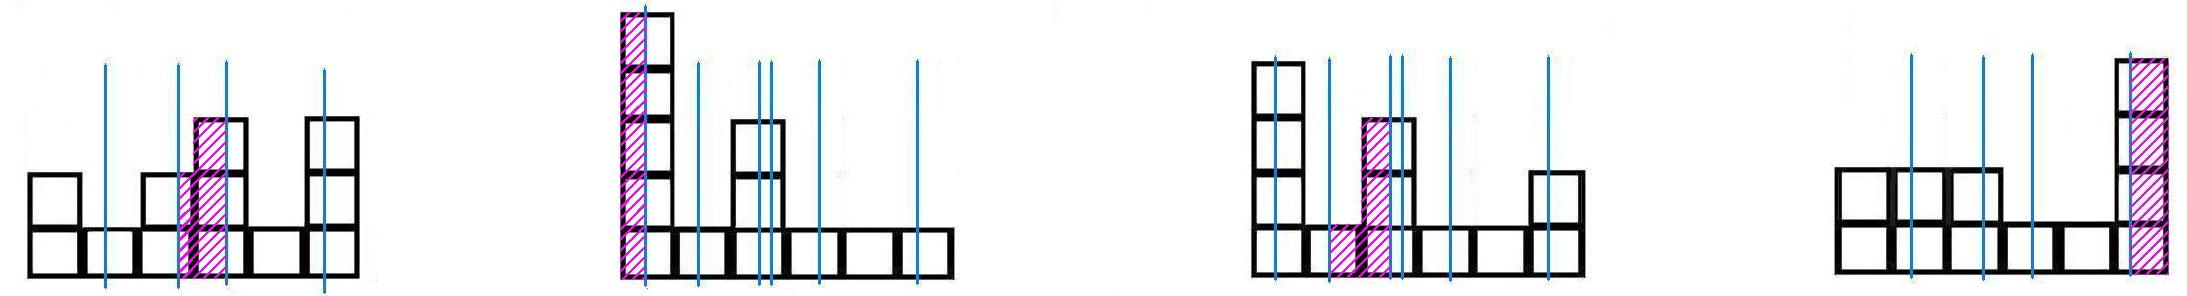
\includegraphics[height=2cm]{upfv5.jpg}
\caption[Beispiel zum unendlichen Protokoll 4/4]{Die Spieler $p_4,p_3,p_2,p_1$ w"ahlen (in dieser Reihenfolge) je ein St"uck aus.}
\end{figure}
\end{bsp}\newpage
\subsection{Ein Absolutum}
Wie wir im Kapitel davor bereits gesehen haben, gibt es auch Protokolle die keine komplette Aufteilung liefern, aber in der Teilaufteilung neidfrei sind. So k"onnte man solche Teilaufteilungen untersuchen und versuchen zu vereinen. Dabei kann man auch von einem vorgegebenen Zustand ausgehen und den Kuchen bis zum Ende aufteilen. Eine solche Teilaufteilung ist hier gebenen:
\begin{defi}{\textbf{(Absolutum)}}
\newline Eine Kuchenaufteilung f"ur vier Spieler ist ein \underline{Absolutum}, falls es eine Aufteilung $\{X_1,X_2,X_3,X_4,R\}$ in einem neidfreien Zustand gibt mit der Eigenschaft, dass jedem Spieler $p_i$  das St"uck $X_i$, $i\in \{1,2,3,4\}$ bereits zugeodnet, und es gilt: Es gibt einen Spieler, so dass $v_i(X_i)>v_i(X_j)+1/2\cdot v_i(R)$ f"ur alle $i,j \in \{1,2,3,4\}, i \neq j$. 
\end{defi}
\begin{satz}
Falls eine Kuchenaufteilung ein Absolutum ist, so existiert eine neidfreie, endlich unbeschr"ankte Aufteilung f"ur vier Spieler.
\end{satz}
\begin{proof}
Falls eine Kuchenaufteilung ein Absolutum ist, so ist sie in einem neidfreien Zustand und es gilt: Es gibt einen Spieler so dass $v_i(X_i)>v_i(X_j)+1/2\cdot R$ f"ur alle $i,j \in \{1,2,3,4\}, i \neq j$. O.B.d.A. sei dies der Spieler $p_1$. Der Spieler $p_1$ schneidet das kleinste St"uck $R_1$ von $X_1$ ab, so dass $v_1(X_1')$=$v_1(X_j)$ f"ur ein beliebiges $j \in \{1,2,3\}$. O.B.d.A. sei dies das St"uck $X_2$. Es gilt $R'=R+R_1$ und $v_1(R_1)>1/3 \cdot v_1(R')$, denn $v_1(X_1)>v_1(X_2)+1/2\cdot v_1(R)$. Sei $R_1'+\epsilon= R_1$ mit der Eigenschaft $v_1(R_1)=1/3 \cdot v_1(R')$. Da $R_1$ urspr"unglich zu $X_1$ geh"ort hat und unsere Teilaufteilung neidfrei war, bekommt $p_1$ $R_1$ ohne Probleme zur"uck. Nun schneidet $p_1$ von $R$ vier gleichwertige St"ucke (n.s.M.) $\{Y_1,Y_2,Y_3,Y_4\}$ ab mit der Eigenschaft, dass $v_1(Y_i)=1/3 \cdot v_1(R_1')$ f"ur alle $i \in \{1,2,3,4\}$. Die Spieler suchen sich nach einem bestimmten Verfahren drei St"ucke aus. Das "ubrige St"uck bekommt $p_1$. Er wiederholt den letzten Schnitt aber f"ur $1/9 \cdot v_1(R_1')$ und dannach f"ur $(1/3)^k \cdot v_1(R_1')$ f"ur $k \geq 3.$ Das $n$ h"angt von der genauen Zahl um wieviel $v_i(X_i)>v_i(X_j)+1/2\cdot R$. Sei dies die Zahl $c$ f"ur  $constant$. Also $c=v_i(X_i)-v_i(X_j)-1/2\cdot R$. Durch diese Zahl $c$ k"onnen wir annehmen, dass die Reihe $\sum_{k=1}^\infty ((1/3)^k) = 1/2$\footnote[1]{Dies ist der Grenzwert der geometrischen Reihe f"ur n=3} $\iff$ $\sum_{k=1}^n ((1/3)^k) + \sum_{k=n+1}^\infty((1/3)^k)=1/2$ $\iff$ $\sum_{k=1}^n ((1/3)^k) = 1/2 - \sum_{k=n+1}^\infty((1/3)^k)$ 
sei $\sum_{k=n+1}^\infty((1/3)^k) =:c$ und zwar genau unsere oben definierte Zahl $c$. Diese Zahl ist kleiner unendlich, da die Reihe $\sum_{k=1}^n ((1/3)^k)$ absolut\footnote[2]{Aus dieser Eigenschaft folgt auch die Namensgebung} konvergiert und somit endlich ist. D.h. jede Teilfolge gestartet von einem $j>1$ bis $\infty$ ist ebenfalls endlich und somit konstant.\\
Damit wurde gezeigt, dass $\sum{k=1}^n(1/3)^k \cdot v_1(R_1')=1/2\cdot v_1(R_1')$. Dies bedeutet, dass der Spieler $p_1$ glaubt genau die H"alfte von dem Rest bekommen zu haben. Und w"urde somit bei der Restaufteilung keinen Mitspieler beneiden, auch wenn dieser den gesamten Rest bekommen w"urde. Nun bleibt zu zeigen, dass der Kuchen komplett aufgeteilt wurde. Aus der Sicht von Spieler $p_1$ gilt:\\
$1/3\cdot v_1(R_1')+c+4\cdot \sum_{k=2}^n(1/3)^k \cdot v_1(R_1')=1/3\cdot v_1(R_1')+4\cdot (\sum_{k=2}^n(1/3)^k \cdot v_1(R_1') +1/4 \cdot c)$$\Rightarrow^{c_2:= 1/4 \cdot c}$ $1/3\cdot v_1(R_1')+4\cdot ( \sum_{k=2}^n(1/3)^k \cdot v_1(R_1') + c_2)= 1/3\cdot v_1(R_1')+4 \cdot (1/2-1/3)\cdot v_1(R_1')= 1/3\cdot v_1(R_1') + 4/6\cdot v_1(R_1') = v_1(R_1')$. Damit ist nach Spieler $p_1$ der gesamte Kuchen aufgeteilt. Und aus der Eigenschaft, dass f"ur alle Spieler eine nicht leere Teilmenge des Kuchens auch einen positiven Wert besitzt, folgt, dass der Kuchen f"ur alle Spieler damit aufgeteilt ist.
\end{proof}
\section{Komplexit"at von Protokollen}
\subsection{Anfragemodell nach J. Robertson und W. Webb}
\textbf{Erinerung:}\\
Ein Protokoll hat am Anfang keine Informationen "uber die Bewertungen der Spieler, bis auf die Normalisierung. Der Kuchen $X$ wird durch das Intervall $[0,1]\subseteq \mathbb{R}$ repr"asentiert. F"ur ein $\alpha \in \mathbb{R}$ mit $0 \leq \alpha \leq 1$ bezeichnet man als ein \underline{$\alpha$-Punkt} vom Spieler $p_i$ f"ur $p_i \in P_N$ die kleinste Zahl $x$ mit der Eigenschaft $v_i([0,x])=\alpha$ (aus den Eigenschaften der Bewertung folgt $v_i([x,1])=1-\alpha$).
\begin{defi}[Anfragen im Robertson-Webb Modell] \wf rgkhbr \tf \\
\begin{itemize}
\item Schnitt($p_i;\alpha$): Der Spieler $p_i$ macht einen Schnitt in seinem $\alpha$-Punkt. Der Wert $x$ wird an das Protokoll zur"uckgegeben.\\
\item Bewertung($p_i;x$): Der Spieler $p_i$ bewertet den Schnitt $x$ ($x$ ist dabei ein Schnitt, welcher zuvor vom Protokoll ausgef"uhrt wurde). Dieser Wert $v_i(x)$ wird an das Protokoll zur"uckgegeben.\\
\item Zuordnung($p_i;x_i,x_j$): Dem Spieler $p_i$ wird das Intervall $[x_i,x_j]$ ($x_i \leq x_j$ sind zwei zuvor ausgef"uhrte Schnitte vom Protokoll oder 0 oder 1) zugeordnet. Alle solche Intervalle sind disjunkt.
\end{itemize}  
\end{defi}
Die \underline{Komplexit"at eines Protokolls} ist die Summe der Anzahlen der Schnitte und Bewertungen im worst case.
\subsection{Resultat von M. Magdon-Ismail, C. Busch und\\M. S. Krishnamoorthy}
Es wurden zwei Theoreme "uber die unteren Schranken von starken und super neidfreien Cake-Cutting-Protokolle in \cite{6} bewiesen.
\begin{thm}(Untere Schranke von starken neidfreien Protokollen)
\newline Es gibt Bewertungsfunktionen, f"ur welche ein starkes neidfreies Cake-Cutting-Protokoll die Komplexit"at $\Omega(0.086\cdot n^2)$ besitzt.
\end{thm}
\begin{thm}(Untere Schranke von super-neidfreien Protokollen)
\newline Es gibt Bewertungsfunktionen f"ur welche ein super-neidfreies Cake-Cutting-Protokoll die Komplexit"at $\Omega(0.25\cdot n^2)$ besitzt.
\end{thm}
Das Resultat zeigt bereits einen Unterschied zu den proportionalen Protokollen ($\mathcal O(n$log$ n)$ aus Even $\&$ Paz), ist aber leider sehr schwach, da starke und super-neidfreien Cake-Cutting-Protokolle sehr starke Einschr"ankungen sind, und nicht immer existieren. Dagegen lieferte das folgende Theorem die lang vermutete endg"ultige Separation von der Proportionalit"at.\\
\newline
\subsection{Resultat von A. Procaccia}
Die Komplexit"at bei der neidfreien Aufteilung muss h"oher sein als bei der proportionalen, da man bei jeder Ver"anderung eines St"uckes jeden beteiligten und unbeteiligten Spieler beachten muss.\rf So l"asst sich diese Eigenschaft, formuliert als ein kompliziertes Problem ausnutzen um $\Omega( n^2)$ als untere Schranke f"ur die Neidfreiheit zu setzen.\tf\\
\newline
%\begin{thm} \wf jbdfksdbfksd\\ \tf
%Die Anfragekomplexit"at (im Robertson- Webb- Modell) f"ur eine neidfreie %Aufteilung betr"agt $\Omega(n^2)$.
%\end{thm}
\textbf{Die Idee:}\\
Die Aufgabe von jedem Spieler ist es einzeln und unabh"angig von den anderen Spielern den Kuchen in Intervalle zu unterteilen. Diese Intervalle werden in $\Pi_k^i$ mit $i \in \mathbb{N}$ f"ur jeweils den $p_i$-ten Spieler und $k \in \mathbb{N}$, f"ur die $k$-te Etappe der Gliederung, dargestellt. Wenn zwei Eigenschaften erf"ullt werden, erfolgt eine Aufteilung der St"ucke unter den Spieler. Die erste Eiigenschaft gilt f"ur die H"alfte der Spieler, welche gew"ahrleisten m"ussen, dass ihre St"ucke, die aus einem oder mehreren Intervallen bestehend, h"ochstens die L"ange $2/n$ haben. Ansonsten h"atte der gesamte Kuchen eine L"ange $>1$. Die zweite Eigenschaft ist die Ausschlaggebendheit (critical). Nur wenn jedes St"uck nach jedem Spieler ausschlaggebend ist, kann eine Aufteilung neidfrei sein. Ein ausschlagebendes St"uck muss aus Intervallen bestehen deren Summe der Werte mindestens so gross ist, wie der Wert jedes anderen Intervalls w"ahrend der Aufteilung. Denn g"abe es ein Intervall, dass mehr Wert ist als unser betrachtetes St"uck, so w"urde es ein Gegenspieler bekommen, und es w"urde Neid entstehen. Jeder Spieler braucht mindestens $n/4$ Ausf"uhrungen der Aufteilung um nur Intervalle mit h"ochstens L"ange $2/n$ zu bekommen. Diese Anzahl folgt aus der Durchf"uhrung, denn es lassen sich h"ochstens zwei zus"atzliche Intervalle in einer Etappe der Gielderung erzeugen. Bevor dies der Fall ist, kann das St"uck des jeweiligen Spieler nicht ausschlaggebend und damit die Aufteilung nicht neidfrei sein. Damit gilt f"ur die Komplexit"at $\Omega(\# Spieler \cdot \# Ausf"uhrungen)=\Omega(n/2 \cdot n/4)=\Omega(n^2)$.\\ Hier wird eine untere Schranke gezeigt, damit kann die tats"achliche Anzahl der Etappen der Gliederung weit aus h"ocher sein, als das hier angegebene Minimum $n/2*n/4$. Dies ist vergleichbar mit einer Dauerangabe einer Wegbeschreibung. Der direkte und k"urzeste Weg ist nicht immer m"oglich, aber nur auf Grund der Entfernung lassen sich die Mindestangaben formulieren. Genauso ist es nichtssagend "uber die k"urzeste Wegdauer, wenn die betrachtete Person zun"achst im Kreis l"auft  und erst dann die Distanz hinterlegt.\\
\newline
\textbf{Veranschaulichung an einem Beispiel:}\\
Man f"uhrt solange Schnitt- und Bewertungsanfragen aus bis mindestens $n/2$ Spieler nur Intervalle der L"ange kleiner gleich $2/n$ haben und diese werden dann auf Ausschlaggebenheit untersucht. Die L"ange der Intervalle muss kleiner gleich der L"ange des St"uckes sein, welches der Spieler bekommt, sein, da jedes St"uck Kuchen die Vereinigung von endlich vielen disjunkten Intervallen ist.\\
\newline
Beispiel f"ur vier Spieler mit mindestens drei Schnitten:(dies ist das Minimum um vier St"ucke zu erhalten): 
\begin{itemize}
\item Ausgangssituation: $\Pi_1^0=\{[0,1]\}$, $\Pi_2^0=\{[0,1]\}$, $\Pi_3^0=\{[0,1]\}$, $\Pi_4^0=\{[0,1]\}$
\item  Schnitt($p_1;1/3$)=$1/4$ \\$\Pi_1^1=\{[0,1/4],[1/4,1]\}$, $\Pi_2^1=\{[0,1]\}$, $\Pi_3^1=\{[0,1]\}$, $\Pi_4^1=\{[0,1]\}$
\item  Schnitt($p_2;1/2$)=$3/4$ \\$\Pi_1^2=\{[0,1/4],[1/4,1]\}$, $\Pi_2^2=\{[0,3/4],[3/4,1]\}$, $\Pi_3^2=\{[0,1]\}$, $\Pi_4^2=\{[0,1]\}$
\item  Bewertung($p_3;[1/4,3/4]$)=$7/8$, Protokoll erf"ahrt zus"atzlich $v_3([0,1/4])=1/16$ und $v_3([3/4,1])=1/16$.\\ $\Pi_1^3=\{[0,1/4],[1/4,1]\}$, $\Pi_2^3=\{[0,3/4],[3/4,1]\}$, $\Pi_3^3=\{[0,1/4],[1/4,3/4],[3/4,1]\}$, $\Pi_4^3=\{[0,1]\}$
\item  Schnitt($p_4;1/2$)=$1/2$ (Das Minimum der Schnitte wurde erreicht.)\\ $\Pi_1^4=\{[0,1/4],[1/4,1]\}$, $\Pi_2^4=\{[0,3/4],[3/4,1]\}$, $\Pi_3^4=\{[0,1/4],[1/4,3/4],[3/4,1]\}$, $\Pi_4^4=\{[0,1/2],[1/2,1]\}$
\item  Bewertung($p_4;[1/4,3/4]$)=$7/10$, Protokoll erf"ahrt zus"atzlich $v_4([0,1/4])=1/10$, $v_4([1/4,1/2])=4/10$, $v_4([1/2,3/4])=3/10$ und $v_3([3/4,1])=2/10$. Damit sind alle Intervalle bewertet und die L"ange aller Intervalle ist kleiner $1/2$. \\ $\Pi_1^5=\{[0,1/4],[1/4,1]\}$, $\Pi_2^5=\{[0,3/4],[3/4,1]\}$, $\Pi_3^5=\{[0,1/4],[1/4,3/4],[3/4,1]\}$, $\Pi_4^5=\{[0,1/4],[1/4,1/2],[1/2,3/4],[3/4,1]\}$
\item Bewertung($p_3;[1/4,1/2]$)=$5/8$, Protokoll erf"ahrt zus"atzlich $v_3([1/2,3/4])=2/8$. Auch hier ist die L"ange kleiner $1/2$. Nun haben wir 2 Spieler mit dieser Eigenschaft und k"onnen eine Aufteilung versuchen und die Ausschlaggebendheit untersuchen.\\ $\Pi_1^6=\{[0,1/4],[1/4,1]\}$, $\Pi_2^6=\{[0,3/4],[3/4,1]\}$, $\Pi_3^6=\{[0,1/4],[1/4,1/2],[1/2,3/4],$\\ $[3/4,1]\}$, $\Pi_4^6=\{[0,1/4],[1/4,1/2],[1/2,3/4],[3/4,1]\}$
\item Der Spieler $p_1$ w"urde das St"uck $X_1$ bekommen. Dieses St"uck ist nicht ausschlaggebend, denn f"ur das Intervall $I_1$ gilt $v_1(X_1)<v_1(I_1)$, damit k"onnten $X_4$ oder $X_3$ mehr Wert sein (n.s.M.). Also f"uhren wir noch einen Schritt aus.
\item  Bewertung($p_1;[1/2,3/4]$)=$1/4$, Protokoll erf"ahrt zus"atzlich $v_1([1/4,1/2])=1/6$ und $v_1([3/4,1])=1/4$ \\ $\Pi_1^7=\{[0,1/4],[1/4,1/2],[1/2,3/4],[3/4,1]\}$, $\Pi_2^7=\{[0,3/4],[3/4,1]\}$, $\Pi_3^7=\{[0,1/4],[1/4,1/2],[1/2,3/4],[3/4,1]\}$, $\Pi_4^7=\{[0,1/4],[1/4,1/2],[1/2,3/4],[3/4,1]\}$
\item Nun sind alle St"ucke ausschlaggebend und "uber die H"alfte der Spieler haben nur Intervalle mit der L"ange kleiner gleich $1/2$. Als liegt einer Aufteilung nichts mehr im Wege und wir f"uhren diese aus.
\begin{figure}[h!]
\center
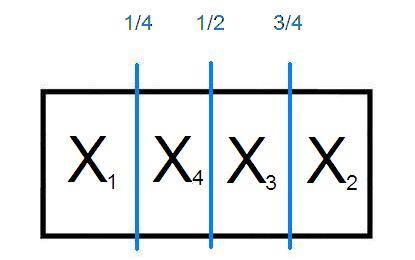
\includegraphics[height=4cm]{kk4.jpg}
\caption[Beispiel zu Procaccias Teilungsspiel]{Die Aufteilung}
\end{figure}  
\end{itemize}
\section{Zusammenfassung und Ausblick}
Es kann untersucht werden, ob einige Protokolle Neid garantieren. Wenn man z.B. dem ersten Spieler seinen proportionalen Anteil zuordnet und davon ausgeht, dass die Bewertungsfunktionen nicht gleich sind, so ist Neid garantiert.\\
Ein weiteres nat"urliches Problem ist die Aufteilung mit Vollmachten. So "ubertragen z.B. ein Teil der Spieler ihre Vollmacht an einen Verantwortlichen, dieser sieht ihre Bewertungen und kann somit Ihnen St"ucke zuordnen. Hier untersuche man, ob die Neidfreiheit leichter oder schwieriger erreicht werden kann. Au"serdem kann nun in Abh"angigkeit der Ehrlichkeit des Verantwortlichen die Effizienz der Aufteilungen gepr"uft werden. Es kann auch gepr"uft werden, wie sich die Aufteilung entwickelt, wenn ein Spieler die Vollmacht von allen Anderen hat. Oder wenn mehrere Spieler Vollmachtbeauftragte sind (z.B. Scheidung und das Kind l"asst beide Eltern f"ur es alles regeln).\\
Es kann untersucht werden, ob die Aufteilung mit offenen Bewertungsfunktionen gleichwertig mit dem Finden eines Nash-Gleichgewichtes ist.\\
\subsection{Simulation durch ein Programm}
Um die Forschungen in diesem Gebiet zu erleichtern, k"onnte ein Computerprogramm mit folgenden Eigenschaften erstellt werden.\\
\newline
\textbf{Spieler}\\
Die Anzahl der Spieler wird am Anfang eingegeben und f"ur jeden der Spieler wird eine eigene Kopie des Kuchens, sowie eine Bewertungsfunktion f"ur den Kuchen die er bekommt erstellt.\\
\newline
\textbf{Kuchen}\\
Der Kuchen wird f"ur jeden Spieler durch zuf"allig verstreute Punkte in dem Bereich des Kuchens (Intervall $[0,1]$) repr"asentiert.\\ Man kann es sich vorstellen, als ob in eine Backform Salz, Zucker, Pfeffer etc. verstreut wird.\\
\newline 
\textbf{Ma"s}\\
Jeder Spieler bewertet ein St"uck Kuchen in Abh"angigkeit von der Anzahl seiner Punkte. Zum Beispiel ist ein Spieler nur am Salz interessiert, ein Anderer nur am Zucker.\\ 
\newline
\textbf{Vorgehensweise}\\
Die einzelnen Schritte des gepr"uften Protokolls werden eingegeben und ausgef"uhrt.\\
\newline
\textbf{Ergebnis}\\
Am Ende ist der gesamte Kuchen aufgeteilt und jeder Spieler bewertet sein St"uck und die St"ucke der Mitspieler. Es wird gepr"uft ob die entstandene Allokation neidfrei ist.\\
\newline
\textbf{Bemerkungen}\\
Es k"onnen Spezialf"alle eingestellt werden z.B. ein Spieler hat nur seine Punkte im Bereich$[0,1/2]$. Somit ist das Programm sehr realit"atsbezogen.\\
Es k"onnen neue Prokolle auf ihre Neidfreiheit gepr"uft werden.\\
Man kann hiermit auch proportionale Protokolle auf neidfreie Erwartungswerte "uberpr"ufen und somit vergleichen.\\ Beispiel: Man l"asst zwei proportionale Protokolle 1000 mal durchlaufen mit stets unterschiedlicher Punkteverteilungen des Kuchens und bekommt an Ende einen Durchschnittswert "uber die Anzahl der Spieler und die H"aufigkeit ihrer Beneidung der Anderen.\\
\newpage
\thispagestyle{empty}
\thispagestyle{plain}
\renewcommand{\refname}{Literaturverzeichnis}
\addcontentsline{toc}{section}{Literaturverzeichnis}
\begin{thebibliography}{9}
\bibitem[Su]{1}
Cloutier,Nyman,Su:
''Two-Player Envy-Free Multi-Cake Division''
\bibitem[Brams and Taylor, 1995]{} S. J. Brams and A. D. Taylor. An
envy-free cake division protocol. \emph{The American Mathematical Monthly}, 102(1):9-18, 1995.
\bibitem[Brams et al., 1997]{5} S. J. Brams, A. D. Taylor, and W. S.
Zwicker. A moving-knife solution to the four-person envy
free cake division problem. \emph{Proceedings of the American
Mathematical Society}, 125(2):547-554, 1997.
\bibitem[Busch et al., 2005]{} C. Busch, M. S. Krishnamoorthy, and
M.Magdon-Ismail. Hardness results for cake cutting. \emph{Bulletin of the EATCS}, 86:85-106, 2005
\bibitem[Edmonds and Pruhs, 2006]{6} J. Edmonds and K. Pruhs. Cake
cutting really is not a piece of cake. In\emph{Proceedings of
the 17th Annual ACM-SIAM Symposium on Discrete Algorithms (SODA)}, pages 271-278, 2006.
\bibitem[Even and Paz, 1984]{3} S. Even and A. Paz. A note on cake-cutting. \emph{Discrete Applied Mathematics}, 7:285-296, 1984.
\bibitem[Robertson and Webb, 1998] J. M. Robertson and W. A.
Webb. \emph{Cake Cutting Algorithms: Be Fair If You Can.} A.
K. Peters, 1998.
\bibitem[Steinhaus, 1948]{} H. Steinhaus. The problem of fair division. \emph{Econometrica}, 16:101-104, 1948.
\bibitem[Stromquist, 1980]{} W. Stromquist. How to cut a cake fairly.
\emph{American Mathematical Monthly}, 87(8):640-644, 1980.
\bibitem[Stromquist, 2008]{} W. Stromquist. Envy-free cake divisions
cannot be found by finite protocols. \emph{The Electronic Journal of Combinatorics}, 15:$\#$R11, 2008.
\bibitem[Woeginger and Sgall, 2007]{} G. J. Woeginger and J. Sgall.
On the complexity of cake cutting. \emph{Discrete Optimization},
4:213-220, 2007.
\bibitem[MIBK03]{} M. Magdon-Ismail, C. Busch, and M. Krishnamoorthy. Cake-cutting is not a piece of cake. In \emph{Proceedings of the 20th Annual Symposium on Theoretical Aspects of Computer Science}, pages
596-607. Springer-Verlag \emph{Lecture Notes in Computer Science} $\#$2607, 2003.
\bibitem[Pro09]{} A. Procaccia. Thou shalt covet thy neighbor's cake. In \emph{Proceedings of the 21st International Joint Conference on Artificial Intelligence}, pages 239-244. IJCAI, July 2009.
\bibitem[BT96]{} S. Brams and A. Taylor. \emph{Fair Division: From Cake-Cutting to Dispute Resolution}. Cambridge University Press, 1996.
\bibitem[BTZ97]{} S. Brams, A. Taylor, and W. Zwicker. A moving-knife solution to the four-person envy-free
cake-division problem. \emph{Proceedings of the American Mathematical Society}, 125(2):547-554,
1997.
\bibitem[Cha85]{} A. Chauduri. Formal properties of interpersonal envy. \emph{Theory and Decision}, 18:301-312, 1985.
\bibitem[EP06b]{} J. Edmonds and K. Pruhs. Cake cutting really is not a piece of cake. In \emph{Proceedings of the 17th
Annual ACM-SIAM Symposium on Discrete Algorithms}, pages 271-278. ACM Press, 2006.
\bibitem[FK74]{} A. Feldman and A. Kirman. Fairness and Envy. \emph{The American Economic Review}, 64(6):995-1005, 1974.
\bibitem[MIBK03]{} M. Magdon-Ismail, C. Busch, and M. Krishnamoorthy. Cake-cutting is not a piece of cake. In \emph{Proceedings of the 20th Annual Symposium on Theoretical Aspects of Computer Science}, pages 596-607. Springer-Verlag Lecture Notes in Computer Science \#2607, 2003.
\bibitem[RW98]{} J. Robertson and W. Webb. \emph{Cake-Cutting Algorithms: Be Fair If You Can}. A K Peters, 1998.
\bibitem[Var74]{} H. Varian. Equity, envy, and efficiency. \emph{Journal of Economic Theory}, 9(1):63-91, 1974.
\bibitem[Ste49]{} H. Steinhaus. Sur la division pragmatique. \emph{Econometrica}, 17:315-319, 1949. Supplement.
\bibitem[Wel85]{} D.Weller. Fair division of a measurable space. \emph{Journal of Mathematical Economics}, 14(1):5-17,
1985.
\bibitem[Su]{1}
Cloutier,Nyman,Su:
''Two-Player Envy-Free Multi-Cake Division''
\bibitem[Su]{1}
Cloutier,Nyman,Su:
''Two-Player Envy-Free Multi-Cake Division''
\bibitem[Su]{1}
Cloutier,Nyman,Su:
''Two-Player Envy-Free Multi-Cake Division''
\bibitem[Su]{1}
Cloutier,Nyman,Su:
''Two-Player Envy-Free Multi-Cake Division''
\bibitem[Su]{1}
Cloutier,Nyman,Su:
''Two-Player Envy-Free Multi-Cake Division''
\bibitem[Su]{1}
Cloutier,Nyman,Su:
''Two-Player Envy-Free Multi-Cake Division''
\bibitem[Su]{1}
Cloutier,Nyman,Su:
''Two-Player Envy-Free Multi-Cake Division''
\bibitem[Su]{1}
Cloutier,Nyman,Su:
''Two-Player Envy-Free Multi-Cake Division''
\bibitem[Su]{1}
Cloutier,Nyman,Su:
''Two-Player Envy-Free Multi-Cake Division''
\bibitem[Su]{1}
Cloutier,Nyman,Su:
''Two-Player Envy-Free Multi-Cake Division''
\bibitem[Su]{1}
Cloutier,Nyman,Su:
''Two-Player Envy-Free Multi-Cake Division''
\bibitem[Su]{1}
Cloutier,Nyman,Su:
''Two-Player Envy-Free Multi-Cake Division''
\bibitem[Su]{1}
Cloutier,Nyman,Su:
''Two-Player Envy-Free Multi-Cake Division''
\bibitem[Su]{1}
Cloutier,Nyman,Su:
''Two-Player Envy-Free Multi-Cake Division''
\bibitem[Su]{1}
Cloutier,Nyman,Su:
''Two-Player Envy-Free Multi-Cake Division''
\bibitem[Su]{1}
Cloutier,Nyman,Su:
''Two-Player Envy-Free Multi-Cake Division''
\bibitem[Su]{1}
Cloutier,Nyman,Su:
''Two-Player Envy-Free Multi-Cake Division''
\end{thebibliography}
\newpage
\thispagestyle{empty}
\tf
\begin{center}
\Huge Erkl"arung
\end{center}
\vspace{1cm}
\noindent Hiermit versichere ich, die vorliegende Bachelorarbeit selbstst"andig verfasst und keine anderen als die angegebenen Quellen und Hilfsmittel benutzt zu haben.\\
\vspace{3cm}\\
D"usseldorf, 21. September 2010 \hfill Alina Elterman

\end{document}
